\chapter[THERMODYNAMIC FAVORABILITY OF THERMOPHILE LIPID CHAIN MODIFICATIONS ACROSS A TEMPERATURE AND REDOX GRADIENT]{Thermodynamic favorability of thermophile lipid chain modifications across a temperature and redox gradient}\label{ch2}

\section{Introduction}

Ongoing efforts are needed to elucidate factors that control lipid distribution in the environment. Our level of understanding ranges widely with respect to how lipid structural adaptations contribute to the biophysical properties or function of the membrane; the roles played by many structures are unknown. Lipids need to function effectively for an organism, and it is plausible that lipid structures that offer the best fitness advantage for the lowest energy cost will be selected over the course of evolution. Chapter \ref{ch1} showed trends in the abundance-weighted average oxidation state of carbon (Z\textsubscript{C}) in observed distributions of intact polar lipids (IPLs) obtained across the temperature and redox gradients of four hot springs in Yellowstone National Park (YNP) offer insight into the natural cost-benefit analysis undergone by thermophilic microorganisms adapted to their surroundings. The abundance-weighted Z\textsubscript{C} of IPLs was shown to increase, \textit{i.e.}, become more oxidized, with decreasing temperature and increasing concentration of dissolved oxygen. The incorporation of proportionally more oxidized carbon into the structures of IPLs downstream was attributed primarily to observed changes in the distributions of alkyl chain structures, such as decreasing chain length, increasing degree of unsaturation, glycerol dialkyl glycerol tetraether (GDGT) chain cyclization, and to switch from ether- to ester-bonded alkyl chain-backbone linkages. With the possible exception of the inclusion of GDGT rings \citep[the function of which is still being explored;][]{sollich2017heat}, these downstream changes in alkyl chain distribution might be interpreted primarily as adaptations to provide thermally tolerant membranes at the temperatures experienced by the microbial communities sampled in these springs. However, I hypothesized in Chapter \ref{ch1} that the alkyl chain modifications providing this membrane thermostability were the result of adaptation to the chemical composition of the surroundings; that more oxidized modifications such as chains with fewer carbons, increased unsaturation and GDGT ring cyclization, and higher fractions of ester linkage were observed under oxidized conditions downstream because these modifications represent a cost-effective solution to providing membrane function in those sets of chemical conditions. Similarly, I argued that more reduced modifications, such as increasing the number of alkyl chain carbons, decreased degree of unsaturation and ring cyclization, and a greater proportion of ether-linkages were more abundant in samples closer to the hot spring source because these modifications were both functional and cost-effective in hot, reduced chemical conditions.

In this study, I performed a thermodynamic investigation into the notion that downstream increase in alkyl chain Z\textsubscript{C} signals an underlying energetic adaptation in microbial membranes to hot spring oxidation-reduction (redox) potential using the same sample set described in Chapter \ref{ch1}. This includes eighteen samples taken across the temperature and chemical gradients of four alkaline hot springs in YNP; Bison Pool (BP), Mound Spring (MS), Empress Pool (EP), and Octopus Spring (OS). Previous thermodynamic studies on the energetic favorability of proteins along the temperature and redox gradient of Bison Pool, YNP \citep{dick2011calculation, dick2013metastable} served as a conceptual foundation for the use of equilibrium assumptions for predicting relative stabilities of biomolecules based on temperature and a set of known geochemical variables. These calculations are based on predicted favorability of reactions to form the biomolecules of interest from `basis species', which in this work were a set of naturally available inorganic aqueous species relevant to autotrophic metabolism and included bicarbonate (HCO\textsubscript{3}\textsuperscript{-}), ammonium (NH\textsubscript{4}\textsuperscript{+}), protons (H\textsuperscript{+}), electrons (e\textsuperscript{-}) and water (H\textsubscript{2}O) for all but one sample that used nitrate (NO\textsubscript{3}\textsuperscript{-}) in place of NH\textsubscript{4}\textsuperscript{+}.

If a biomolecule is predicted to be more stable relative to others of its kind, this might indicate that the biological energy requirement for assembling this biomolecule out of available materials (basis species) is the most cost-effective evolutionary option within the set of geochemical conditions. Likewise, the stability of entire biomolecular assemblages can be assessed so long as thermodynamic properties for individual compounds exist or can be estimated. I wanted to explore whether observed distributions of IPL alkyl chains represented stable, cost-effective assemblages in the context of hot spring temperature and chemical composition. I reasoned that if the alkyl chains sampled from high-temperature, reduced conditions were predicted to be most stable in those conditions relative to the alkyl chains sampled from other sites, and \textit{vice versa} for oxidized conditions, then this would provide evidence of energetically driven convergence on functional lipids.

The thermodynamic properties of alkyl chains first had to be obtained, but the scarcity of experimentally derived data in the literature presented a challenge. Methods exist for estimating properties of organic molecules like alkyl chains (described later) assuming the chemical structures are known, but the structures of individual alkyl chains cannot be resolved with the analytical method used to quantify IPLs in Chapter \ref{ch1}. This inspired the use of `sample-averaged free alkyl chains' (alkyl\textsubscript{free}) as a model for observed lipid distributions in a sample.

\afterpage{
\singlespace
\begin{figure}[h]
\centering
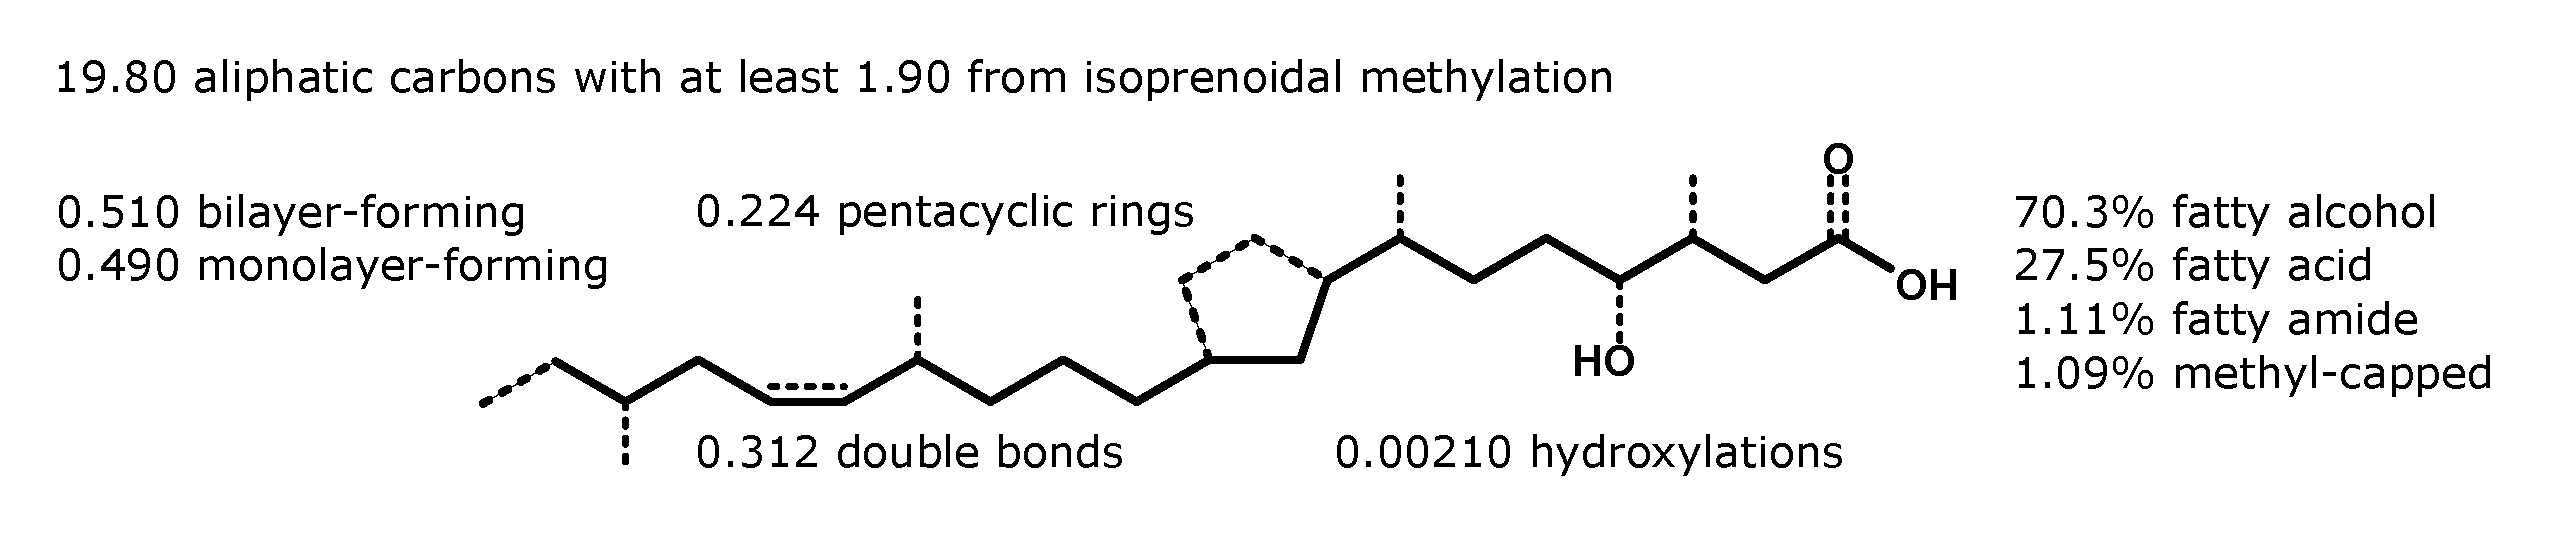
\includegraphics[width=\linewidth]{figs_ch2/sample_average_chain_Bison1}
\caption[Hypothetical chemical structure of the sample-averaged free alkyl chain of Bison Pool sample BP1]{Hypothetical chemical structure of the sample-averaged free alkyl chain (alkyl\textsubscript{free}) of Bison Pool sample BP1 based on abundance-weighted structural characteristics of alkyl chains linked to observed intact polar lipids. Position and isomerism of hydroxylations, pentacyclic rings, methyl branches, and double bonds are not considered when calculating thermodynamic properties of alkyl\textsubscript{free}; their depiction here is to illustrate one of many possible interpretations of a hypothetical average molecule.}
\label{fig:ave_chain}
\end{figure}
\doublespace
\clearpage
}

\afterpage{
\singlespace
\begin{figure}[h]
\centering
\includegraphics[width=\linewidth]{"figs_ch2/linked vs free alkyl chains"}
\caption[Comparison of IPL backbone-alkyl chain linkage types and the free alkyl chains used in thermodynamic calculations]{Comparison of IPL backbone-alkyl chain linkage types (left) and the free alkyl chains used in the thermodynamic calculations of this study (right). R\textsubscript{1} indicates the rest of the alkyl chain and R\textsubscript{2} stands for the remainder of the backbone, headgroup, and other alkyl chains of the IPL. As a part of the thermodynamic estimations performed in this study, abundance-weighted chemical formulae and structures of IPL-linked alkyl chains (orange box, given in Chapter \ref{ch1}) were capped with the elemental and thermodynamic contribution of groups in the yellow box according to alkyl chain-backbone linkage type, arriving at `free' sample-averaged alkyl chains as a model for sample lipid distributions.}
\label{fig:linked_vs_free_chain}
\end{figure}
\doublespace
\clearpage
}


Various abundance-weighted structural characteristics of alkyl chains such as nC (number of aliphatic carbons), nUnsat (number of unsaturations), nOH (number of secondary hydroxylations), mole fraction of monolayer-forming chains and backbone-chain linkage types (ether, ester, amide, and C-C) were calculated from observed abundances of IPLs reported in Table \ref{tab:mods} of Chapter \ref{ch1}. In this study, partial molal thermodynamic aqueous properties of eighteen hypothetical `sample-averaged' alkyl chains were estimated, each representing the abundance-weighted structural characteristics of alkyl chains in a hot spring sample. For instance, the nC and nUnsat in sample BP1 were observed to be 19.80 and 3.12$\times$10\textsuperscript{-1}, respectively, so the thermodynamic properties estimated for the aqueous sample-averaged alkyl chain representing BP1 assume a hypothetical chemical structure with 19.80 aliphatic carbons and 3.12$\times$10\textsuperscript{-1} unsaturations, and so on. A chemical cartoon is shown in Figure \ref{fig:ave_chain} to help visualize how the hypothetical structure of the sample-averaged alkyl chain might look. This is equivalent to calculating thermodynamic properties for thousands of individual chains and then taking an abundance-weighted average of each property. It would not have been possible in this study to estimate the thermodynamic properties of every observed chain due to an inability to resolve structural characteristics of individual IPL alkyl chains using this LC-MS method. The rationale for calculating thermodynamic properties from abundance-weighted structural characteristics was as follows: if an IPL observed in a sample has 38 aliphatic carbons and two unsaturations distributed between two chains, the structural characteristics of its chains must be described using averages without resorting to assumptions about which chain bears which combination of characteristics, and by extension, the estimated thermodynamic properties of alkyl chains must therefore be described by averages as well. This was taken a step further by assuming that the structural characteristics of all alkyl chains in a sample could be averaged for the sake of calculating thermodynamic properties, resulting in the concept of a `sample-averaged' alkyl chain.

In this work, thermodynamic properties were estimated for `free' alkyl chains, as opposed to IPL-linked chains, to provide a simpler model for representing lipid distribution. The difference between IPL-linked and free alkyl chains is represented in Figure \ref{fig:linked_vs_free_chain} for ether-, ester-, amide-, and C-C-linked chains. Except for the C-C linkage type, free chains represent a hydrolyzed version of the IPL-linked chains, with fatty acids, alcohols, and amides corresponding to the free versions of IPL-linked esters, ethers, and amide-bonded alkyl chains. In the case of C-C-linked alkyl chains, the free chain was methyl-capped to maintain alkane-like properties.


A study by \cite{shock1990calculation} demonstrated that the partial molal thermodynamic properties of aqueous hydrocarbons tend to have a strong linear correlation with chain length, as was shown for 1-alkynes, n-alkyl benzenes, 1-alkenes, 1-amines, n-alkanes, aldehydes, 1-alcohols, 2-ketones, methyl alkanoates, n-carboxylic acids, and n-carboxylate ions. This observation served as a theoretical foundation for estimating properties of aqueous alkyl\textsubscript{free} with non-integer values for nC in this work. If a thermodynamic property is linearly correlated with chain length, it should make no difference whether a chain length of 19.0 or 19.8 is used to solve for the value of the property.

\cite{shock1990calculation} also showed thermodynamic properties regressed against chain length were approximately parallel for different functional group chains and differed only by y-intercept. Because the slopes of these regressions were nearly identical, each additional -CH\textsubscript{2}- group was suggested to contribute the same change in the value of the property. This strongly suggests an additive nature for both functional groups and -CH\textsubscript{2}- in linear organic molecules.

This theory of adding together the contribution of individual chemical groups to arrive at the estimated properties of the entire molecule, or `group additivity', is not new. \cite{sugden1924cxlii} showed a property related to surface tension, parachor, could be estimated by group additivity for a variety of organic and inorganic compounds, as well as for a few elements. \cite{benson1958additivity} noted that various group additivity rules were cropping up in the literature and proposed a series generalized of rules for estimating thermodynamic properties of ideal gases, including heat capacity, entropy, and heat of formation from the elements. Studies by \cite{cabani1981group, cabani1977volume2, cabani1977volume1} measured volumetric and thermodynamic properties of aqueous molecules and calculated group contribution values of functional groups. Since then, group additivity has been used to estimate the properties of a great many aqueous organic molecules that lack experimentally measured values.

According to group additivity theory, the thermodynamic contribution of one functional group to a molecule is expected to be roughly the same for each addition. This suggests a linear trend in the estimated property as a function of the number of times the functional group is added, just as was described above for CH\textsubscript{2} groups. Following the same reasoning that was applied to estimating the properties of a chain with a non-integer nC, I estimated the contributions of non-integer unsaturations, hydroxylations, GDGT cyclic rings, isoprenoidal branching to the thermodynamic properties of alkyl\textsubscript{free}. The fractional contributions of the carboxylic acid, alcohol, methyl-capped, and amide functional group of alkyl\textsubscript{free} were also estimated using these guidelines.

\section{Methods}
\subsection{Analysis of water chemistry}
Sampling locations were measured and water samples were collected, filtered, and analyzed as described in Chapter \ref{ch1}. Briefly, temperature and pH were measured in the field as close to the sampling locations as possible using a YSI 30 conductivity meter for temperature and a model 3300i or 3110 WTW pH meter with WTW probe for pH. Concentrations of dissolved oxygen and sulfide were measured in unfiltered water samples using Hach 2400 or 2800 portable spectrophotometer with Hach reagents. Water samples collected for later laboratory analyses were filtered with Supor\textsuperscript{TM} (Pall Corporation) polyethersufone (PES) filters down to 0.2 $\mu$m; samples for ion chromatography were collected in 30 mL HDPE Nalgene bottles (two per sample) and stored at -20$^{\circ}$C before analysis on Dionex DX-600 IC systems for concentrations of major cations and anions.

Filtered samples for dissolved inorganic carbon (DIC) analysis were collected in acid-washed amber glass vials with black butyl rubber septa. DIC was chemically converted to CO\textsubscript{2} by reacting with phosphoric acid before analysis on an OI Wet Oxidation TOC analyzer coupled to a Thermo Delta Plus Advantage mass spectrometer as described in \cite{havig2011merging}.

The Eh of water samples was calculated using measured concentrations of major dissolved solutes and hot spring temperatures using EQ3/6 aqueous geochemical speciation software version 8.0a \citep{wolery2002eq3} and thermodynamic data from the slop16 database available for download at the URL http://geopig.asu.edu/sites/default/files/slop16.dat.

\subsection{Analysis of environmental IPLs} Methods used to collect, identify, and quantify the hot spring microbial IPLs from sediments and biofilms are described in detail in Chapter \ref{ch1}. Briefly, sediments and biofilms were collected into sterile specimen containers with sterilized forceps and spatulas, and stored on dry ice the field, and at -80$^{\circ}$C after transport to the lab. Samples were freeze-dried, homogenized with mortar and pestle, lipids were extracted using a modified version of the Bligh and Dyer method \citep{white1998signature}. Aliquots of the resulting total lipid extracts (TLEs) were analyzed using the hydrophilic interaction chromatography (HILIC) method \citep{wormer2013application} on an Agilent 1200 series high-performance liquid chromatograph (HPLC) attached to an Agilent 6520 Accurate-Mass Quadrupole Time-of-Flight Mass Spectrometer with an electrospray ionization source operated in positive ion mode. Commercially available standards were used to obtain response factors for calculating IPL mole fractions from mass spectral peak areas. Response factors are given in Table \ref{tab:RF} and peak assignments to observed IPLs is reported in Table \ref{tab:IPL}.

\subsection{Deriving properties and chemical formulae of alkyl\textsubscript{free}}

\afterpage{
\singlespace
\begin{table}
\centering
% \begin{adjustbox}{width=\textwidth,keepaspectratio}
\begin{threeparttable}
  \caption{Summary of abundance-weighted structural characteristics of isoprenoidal alkyl chains.}

% Table generated by Excel2LaTeX from sheet 'leftover isoprenoidal props'
\begin{tabular}{clllcc}
\toprule
Site  & Sample & \multicolumn{1}{c}{$x_{AR}$\rtr{leftover_xAR}} & \multicolumn{1}{c}{$x_{GDGT}$\rtr{leftover_xGDGT}} & nPent\rtr{leftover_nPent} & nHex\rtr{leftover_nHex} \\
\midrule
Bison & BP1   & 1.98$\times 10$\textsuperscript{-2} & 4.90$\times 10$\textsuperscript{-1} & 2.24$\times 10$\textsuperscript{-1} &  \\
Pool  & BP2   & 2.30$\times 10$\textsuperscript{-2} & 3.00$\times 10$\textsuperscript{-1} & 1.63$\times 10$\textsuperscript{-1} &  \\
      & BP3   & 1.49$\times 10$\textsuperscript{-3} & 8.81$\times 10$\textsuperscript{-2} & 6.19$\times 10$\textsuperscript{-2} &  \\
      & BP4   &       & 7.16$\times 10$\textsuperscript{-3} & 5.52$\times 10$\textsuperscript{-3} &  \\
      & BP5   & 5.06$\times 10$\textsuperscript{-6} & 7.20$\times 10$\textsuperscript{-4} & 5.69$\times 10$\textsuperscript{-4} &  \\
      & BP6   &       & 2.94$\times 10$\textsuperscript{-3} & 2.40$\times 10$\textsuperscript{-3} &  \\
      &       &       &       &       &  \\
Mound & MS1   &       & 9.99$\times 10$\textsuperscript{-1} & 6.16$\times 10$\textsuperscript{-1} & 2.68$\times 10$\textsuperscript{-3} \\
Spring & MS2   & 2.30$\times 10$\textsuperscript{-2} & 6.07$\times 10$\textsuperscript{-1} & 3.01$\times 10$\textsuperscript{-1} &  \\
      & MS3   &       & 1.64$\times 10$\textsuperscript{-1} & 1.13$\times 10$\textsuperscript{-1} &  \\
      & MS4   &       & 5.85$\times 10$\textsuperscript{-2} & 4.25$\times 10$\textsuperscript{-2} &  \\
      & MS5   &       & 1.09$\times 10$\textsuperscript{-2} & 9.65$\times 10$\textsuperscript{-3} &  \\
      &       &       &       &       &  \\
Empress & EP1   & 1.97$\times 10$\textsuperscript{-2} & 8.63$\times 10$\textsuperscript{-1} & 4.45$\times 10$\textsuperscript{-1} & 1.09$\times 10$\textsuperscript{-2} \\
Pool  & EP2   & 4.74$\times 10$\textsuperscript{-3} & 4.71$\times 10$\textsuperscript{-1} & 2.91$\times 10$\textsuperscript{-1} & 7.83$\times 10$\textsuperscript{-3} \\
      & EP3   & 2.21$\times 10$\textsuperscript{-3} & 6.06$\times 10$\textsuperscript{-1} & 3.61$\times 10$\textsuperscript{-1} & 1.15$\times 10$\textsuperscript{-2} \\
      & EP4   & 4.08$\times 10$\textsuperscript{-3} & 2.31$\times 10$\textsuperscript{-1} & 1.43$\times 10$\textsuperscript{-1} & 2.98$\times 10$\textsuperscript{-3} \\
      & EP5   & 2.78$\times 10$\textsuperscript{-3} & 1.26$\times 10$\textsuperscript{-1} & 7.19$\times 10$\textsuperscript{-2} & 1.12$\times 10$\textsuperscript{-3} \\
      &       &       &       &       &  \\
Octopus & OS1   & 1.26$\times 10$\textsuperscript{-1} & 4.21$\times 10$\textsuperscript{-1} & 1.20$\times 10$\textsuperscript{-1} &  \\
Spring & OS2   & 5.08$\times 10$\textsuperscript{-6} & 7.60$\times 10$\textsuperscript{-3} & 4.21$\times 10$\textsuperscript{-3} & 1.46$\times 10$\textsuperscript{-4} \\
\bottomrule
\end{tabular}%

  
  \begin{tablenotes}
    % The order of footnotes here will determine their letter in the table
    \item Note: a blank value indicates that the structural characteristic was not detected in alkyl chains in the sample.
    
    \tr{leftover_xAR} Mole fraction of alkyl chains belonging to archaeol,
    \tr{leftover_xGDGT} mole fraction of alkyl chains belonging to glycerol dialkyl glycerol tetraethers,
    \tr{leftover_nPent} weighted average number of cyclopentane rings per alkyl chain,
    \tr{leftover_nHex} weighted average number of cyclohexane rings per alkyl chain.
        
  \end{tablenotes}
  
  \label{tab:leftover_props}
  \end{threeparttable}
%   \end{adjustbox}
\end{table}
\setcounter{tabcounter}{0} % reset custom table footnote counter
\doublespace
\clearpage
}

Calculation of the elemental abundance of alkyl\textsubscript{free} began with the chemical formulae of sample-averaged IPL-linked alkyl chains, to which additional carbon, hydrogen, oxygen, and nitrogen were added to convert ether-linked chains into free fatty alcohols, ester-linked chains into free fatty acids, amide-linked chains into free fatty amides, and C-C-linked chains into free methyl-capped chains. Chemical formulae of sample-averaged IPL-linked alkyl chains and mole fractions of alkyl chain linkage types required for these calculations are reported in Table \ref{tab:leftover_props} for isoprenoidal chains and in Table \ref{tab:mods} of Chapter \ref{ch1} for all others.

The number of carbon atoms ($c_{free}$) in the chemical formulae of alkyl\textsubscript{free} was calculated with:

\begin{equation}
    c_{free} = c_{linked} + x_{cc},
\end{equation}

\noindent where $c_{linked}$ indicates the number of carbon atoms in the sample-averaged IPL-linked alkyl chain of the sample, and $x_{cc}$ stands for the observed mole fraction of C-C-linked alkyl chains. Addition of a number of carbons equal to $x_{cc}$ to $c_{linked}$ accounts for the carbon that would be gained with a terminal methyl group, assuming hypothetical carbon-carbon bond breakage of C-C-linked alkyl chains to produce the sample-averaged free chains considered in this study.

The number of hydrogen atoms ($h_{free}$) in the chemical formulae of alkyl\textsubscript{free} was calculated from

\begin{align}
\begin{split}
    h_{free} = &h_{linked} + x_{ether} + x_{ester} + 2(x_{amide}) + 3(x_{cc}), \\
\end{split}
\end{align}

\noindent where $h_{linked}$ represents the number of hydrogen atoms in the sample-averaged IPL-linked alkyl chain of the sample, and $x_{ether}$, $x_{ester}$, and $x_{amide}$ correspond to the observed mole fractions of ether-, ester-, and amide-linked alkyl chains, respectively. A number of hydrogens equal to $x_{ether}$ and $x_{ester}$ are added to $h_{linked}$ to account for the single hydrogen in the hydroxyl groups of the resulting alcohol and carboxylic acid group assuming hypothetical hydrolysis of ether- and ester-linked chains to produce free fatty acids and fatty alcohols. Similarly, two times $x_{amide}$ is added to account for the two hydrogen atoms in the amine group of the free amide after the hypothetical hydrolysis of an amide-linked chain. Lastly, adding a number of hydrogens equal to three times $x_{cc}$ accounts for the three hydrogen atoms added by a terminal methyl group after the hypothetical carbon-carbon breakage of a C-C-linked alkyl chain.

The number of nitrogen atoms ($n_{free}$) in the chemical formulae of alkyl\textsubscript{free} was calculated as

\begin{equation}
    n_{free} = n_{linked} + x_{amide},
\end{equation}

\noindent where $n_{linked}$ indicates the number of nitrogen atoms in the sample-averaged IPL-linked alkyl chain. A number of nitrogen atoms equal to $x_{amide}$ are added to $n_{linked}$ to account for the single nitrogen atom added by the amine group of the free amide after hypothetical hydrolysis of an amide-linked alkyl chain.

The number of oxygen atoms ($o_{free}$) in the chemical formulae of alkyl\textsubscript{free} was calculated with

\begin{equation}
    o_{free} = o_{linked} + x_{ether} + x_{ester},
\end{equation}

\noindent where $o_{linked}$ is the number of oxygen atoms in the sample-averaged IPL-linked alkyl chain. A number of oxygen atoms equal to $x_{ether}$ and $x_{ester}$ are added to $o_{linked}$ to account for the single oxygen atom in the hydroxyl groups of the resulting alcohol and carboxylic acid group assuming hypothetical hydrolysis of ether- and ester-linked chains to produce free fatty acids and fatty alcohols.

\subsection{Calculation of thermodynamic properties}

\afterpage{
\singlespace
\begin{table}
\centering
\begin{adjustbox}{width=0.7\linewidth,keepaspectratio}
\begin{threeparttable}
  \caption{Partial molal thermodynamic aqueous and hydration properties of aliphatic carboxylic acids, alcohols, and alkanes with nC $>$ 2 used in the estimation of saturated fatty acid, fatty alcohol, and fatty hydrocarbon properties.}



% Table generated by Excel2LaTeX from sheet 'linkage thermo table'
\begin{tabular}{lrrrrr}
\toprule
      & $\Delta_{f}G^{\circ}_{aq}$\rtr{linkage_kjpermol} & $\Delta_{f}H^{\circ}_{aq}$\rtr{linkage_kjpermol} & $Cp^{\circ}_{aq}$\rtr{linkage_jpermolk} & $V^{\circ}_{aq}$\rtr{linkage_cm3permol} & $\Delta_{h}G^{\circ}$\rtr{linkage_kjpermol} \\
\midrule
\textit{carboxylic acids\rtr{linkage_from_shock1995}} &       &       &       &       &  \\
propanoic acid & -390.99 & -512.41 & 253   & 67.9  & -21.4\rtr{khan1992henry} \\
n-butanoic acid & -381.62 & -535.34 & 337   & 84.61 & -20.9\rtr{khan1992henry} \\
n-pentanoic acid & -373.38 & -559.36 & 432.2 & 100.5 & -19.0\rtr{khan1992henry} \\
n-hexanoic acid & -364.51 & -582.79 & 523.0 & 116.55 & -17.8\rtr{khan1992henry} \\
n-heptanoic acid & -356.48 & -607.01 & 611.7 & 131.6 & -\rtr{linkage_missing} \\
n-octanoic acid & -349.15 & -631.99 & 700.4 & 147.4 & - \\
n-nonanoic acid & -339.82 & -654.92 & 789.1 & 163.2 & - \\
n-decanoic acid & -331.25 & -678.64 & 877.8 & 179.0 & - \\
n-undecanoic acid & -322.71 & -702.37 & 966.5 & 194.8 & - \\
n-dodecanoic acid & -314.13 & -726.09 & 1055  & 210.6 & - \\
      &       &       &       &       &  \\
\textit{1-alcohols\rtr{linkage_from_ORCHYD}} &       &       &       &       &  \\
1-propanol & -172.07 & -312.74 & 355   & 70.71 & -12.36 \\
1-butanol & -162.40 & -336.53 & 443   & 86.53 & -11.86 \\
1-pentanol & -151.72 & -359.56 & 535   & 102.50 & -11.11 \\
1-hexanol & -143.31 & -383.79 & 617   & 118.46 & -10.30 \\
1-heptanol & -134.41 & -408.39 & 702   & 133.03 & -9.72 \\
1-octanol & -123.93 & -429.85 & 778   & 151.20 & -9.14 \\
1-nonanol & -115.24 & -454.67 & 865   & 164.55 & -8.36 \\
1-decanol & -106.23 & -478.75 & 950   & 180.16 & -8.18 \\
1-undecanol & -96.52 & -502.77 & 1034  & 195.77 & -6.90 \\
1-dodecanol & -86.17 & -525.73 & 1119  & 211.38 & -6.04 \\
      &       &       &       &       &  \\
\textit{alkanes\rtr{linkage_from_ORCHYD}} &       &       &       &       &  \\
propane & -8.22 & -127.43 & 398   & 69.31 & 16.09 \\
n-butane & 0.24  & -151.53 & 482   & 75.55 & 16.58 \\
n-pentane & 8.88  & -175.45 & 573   & 99.07 & 17.52 \\
n-hexane & 19.26 & -198.69 & 636   & 114.68 & 18.26 \\
n-heptane & 27.45 & -224.54 & 739   & 130.29 & 18.95 \\
n-octane & 36.08 & -250.45 & 824   & 145.90 & 19.64 \\
n-nonane & 46.24 & -275.24 & 908   & 161.51 & 20.51 \\
n-decane & 55.50 & -296.34 & 993   & 177.12 & 21.24 \\
n-undecane & 64.71 & -321.12 & 1078  & 192.73 & 22.94 \\
n-dodecane & 74.65 & -343.26 & 1163  & 208.34 & 22.51 \\
n-tridecane & 81.58 & -368.84 & 1248  & 223.95 & 22.87 \\
n-tetradecane & 90.85 & -392.99 & 1333  & 239.56 & 23.55 \\
\bottomrule
\end{tabular}%





  
  \begin{tablenotes}
    % The order of footnotes here will determine their letter in the table
    \tr{linkage_kjpermol} kJ mol\textsuperscript{-1},
    \tr{linkage_jpermolk} J mol\textsuperscript{-1} K\textsuperscript{-1},
    \tr{linkage_cm3permol} cm\textsuperscript{3} mol\textsuperscript{-1},
    \tr{linkage_from_shock1995} carboxylic acid properties are taken from \cite{shock1995organic} unless otherwise noted,
    \tr{khan1992henry} values calculated from Henry's law constants, $K_{H}$, reported in \cite{khan1992henry} using the relation $\Delta_{h}G^{\circ} = -RT\ln{K_{H}}$,
    \tr{linkage_missing} indicates a value that was not found in the literature,
    \tr{linkage_from_ORCHYD} properties for alcohols and alkanes are recommended values from the ORganic Compounds HYDration properties (ORCHYD) database compiled by \cite{plyasunova2004database}.

        
  \end{tablenotes}
  
  \label{tab:carbacid_alc_alk_props}
  \end{threeparttable}
  \end{adjustbox}
\end{table}
\setcounter{tabcounter}{0} % reset custom table footnote counter
\doublespace
\clearpage
}


\afterpage{
\singlespace
\begin{table}
\centering
\begin{threeparttable}
  \caption{Regression statistics for partial molal properties of fatty acids, fatty alcohols, and alkanes with nC $>$ 2 as a function of carbon length.}


% Table generated by Excel2LaTeX from sheet 'linkage regress table'
\begin{tabular}{llrrrr}
\toprule
property & chain type & slope & intercept & R\textsuperscript{2} & p-value\rtr{regress_pval} \\
\midrule
$\Delta_{f}G^{\circ}_{aq}$\rtr{regress_kjpermol} & fatty acid & 8.46  & -415.87 & $>$0.99 & $<$0.01 \\
      & fatty alcohol & 9.43  & -199.95 & $>$0.99 & $<$0.01 \\
      & alkane & 9.10  & -35.95 & $>$0.99 & $<$0.01 \\
\midrule
$\Delta_{f}H^{\circ}_{aq}$\rtr{regress_kjpermol} & fatty acid & -23.82 & -440.45 & $>$0.99 & $<$0.01 \\
      & fatty alcohol & -23.70 & -241.52 & $>$0.99 & $<$0.01 \\
      & alkane & -24.14 & -55.30 & $>$0.99 & $<$0.01 \\
\midrule
$Cp^{\circ}_{aq}$\rtr{regress_jpermolk} & fatty acid & 89    & -15   & $>$0.99 & $<$0.01 \\
      & fatty alcohol & 84    & 108   & $>$0.99 & $<$0.01 \\
      & alkane & 85    & 140   & $>$0.99 & $<$0.01 \\
\midrule
$V^{\circ}_{aq}$\rtr{regress_cm3permol} & fatty acid & 15.8  & 21.3  & $>$0.99 & $<$0.01 \\
      & fatty alcohol & 15.61 & 24.36 & $>$0.99 & $<$0.01 \\
      & alkane & 15.80 & 18.84 & $>$0.99 & $<$0.01 \\
\midrule
$\Delta_{h}G^{\circ}$\rtr{regress_kjpermol} & fatty acid & 1.3   & -25.5 & 0.96  & 0.021 \\
      & fatty alcohol & 0.68  & -14.52 & 0.99  & $<$0.01 \\
      & alkane & 0.72  & 13.97 & 0.98  & $<$0.01 \\
\bottomrule
\end{tabular}%



  
  \begin{tablenotes}
    % The order of footnotes here will determine their letter in the table
    Regressed thermodynamic properties are given in Table \ref{tab:carbacid_alc_alk_props}.
    
    \tr{regress_pval} F-test p-value for linear model,
    \tr{regress_kjpermol} kJ mol\textsuperscript{-1},
    \tr{regress_jpermolk} J mol\textsuperscript{-1} K\textsuperscript{-1},
    \tr{regress_cm3permol} cm\textsuperscript{3} mol\textsuperscript{-1}
    
        
  \end{tablenotes}
  
  \label{tab:regress_chain_prop}
  \end{threeparttable}
\end{table}
\setcounter{tabcounter}{0} % reset custom table footnote counter
\doublespace
\clearpage
}



Thermodynamic properties for alkyl\textsubscript{free} were estimated assuming the species were in the aqueous phase. The standard state convention for species in the aqueous phase assumed unit activity in a hypothetical 1 mol$\times$kg$^{-1}$ solution referenced to infinite dilution at any temperature and pressure. The standard state used for liquid water was one unit activity of pure H$_{2}$O at any temperature and pressure. The standard state used for gaseous species was unit fugacity of the ideal gas at 1 bar and any temperature. Hydration properties were chosen to reflect the equilibrium process of transferring 1 mole of the species in the gas phase to the aqueous phase \citep{plyasunov2000thermodynamic}.

Aqueous partial molal thermodynamic Gibbs free energies and enthalpies of formation from the elements ($\Delta_{f}G_{aq}^{\circ}$ and $\Delta_{f}H_{aq}^{\circ}$, respectively), volumes ($V_{aq}^{\circ}$), heat capacities ($Cp_{aq}^{\circ}$), and Gibbs free energies of the hydration process ($\Delta_{h}G^{\circ}$) were estimated for alkyl\textsubscript{free} in two steps. The goal of the first step was to estimate the properties of a saturated, straight aliphatic chain of length nC, terminating at one end with a hybrid functional group. This hybrid group was a combination of alcohol, carboxylic acid, alkane, and amide, with the fraction of each set by observed mole fractions of ether, ester, C-C, and amide-linked IPL alkyl chains, respectively. 

Experimentally derived thermodynamic properties of carboxylic acids, primary alcohols, and alkanes were gathered from the literature into Table \ref{tab:carbacid_alc_alk_props} and then regressed as a linear function of chain length. The results of these regressions are shown in Table \ref{tab:regress_chain_prop}. Properties for n-amides were not readily available and were estimated using a different method, described later.
The slopes and intercepts of these regressions were used to estimate the properties of a hybrid fatty alkyl chain, $\Xi_{fatty}$, according to the equation:

\begin{align}
\begin{split}
\Xi_{fatty} = & (m_{alcohol}\cdot \text{nC} + b_{alcohol})(x_{ether}) \\
            + & (m_{acid}\cdot \text{nC} + b_{acid})(x_{ester}) \\
            + & (m_{alkane}\cdot \text{nC} + b_{alkane})(x_{cc}) \\
            + & (m_{acid}\cdot \text{nC} + b_{acid} + \Delta\Xi_{amide})(x_{amide}), \\
\end{split}
\end{align}

\noindent where $m_{alcohol}$, $m_{acid}$, $m_{alkane}$, $b_{alcohol}$, $b_{acid}$, and $b_{alkane}$ correspond to the slopes ($m$) and intercepts ($b$) of linear regressions of the value of each thermodynamic property as a function of chain length for fatty acids, fatty alcohols, and alkanes. Mole fractions of ether-linked, ester-linked, C-C-linked, and amide-linked alkyl chains observed in the sample are indicated by $x_{ether}$, $x_{ester}$, $x_{cc}$, and $x_{amide}$, respectively. The estimated difference in the thermodynamic property between a fatty amid and fatty acid is represented by $\Delta\Xi_{amide}$, given in Table \ref{tab:amide}. The first three terms of this equation use the slopes and intercepts of the regression of the property of interest to obtain the property of a straight fatty chain with a length equal to nC, and then weights the contributions of those properties by the mole fractions of observed IPL alkyl chain linkages; fatty alcohols, fatty acids, and fatty alkanes are weighted by the mole fractions of ethers, esters, and C-C linked alkyl chains, respectively. In the fourth term of the equation, a carboxylic acid of length nC was instead estimated by $m_{acid}\cdot \text{nC} + b_{acid}$, to which $\Delta\Xi_{amide}$ was added to convert the carboxylic acid into an amide. The contribution of fatty amides to $\Xi_{fatty}$ was not estimated by regression of aqueous amide properties in the same way as alcohols, carboxylic acids, and alkanes due to a lack of literature data, necessitating the carboxylic acid to amide correction, \textit{i.e.}, $\Delta\Xi_{amide}$.


\afterpage{
\singlespace
\begin{table}
\centering
% \begin{adjustbox}{width=\textheight,keepaspectratio}
\begin{threeparttable}
  \caption{Partial molal thermodynamic aqueous and hydration properties of functional groups and chemical species used in the estimation of fatty amide properties.}



% Table generated by Excel2LaTeX from sheet 'fatty amide table'
\begin{tabular}{lrrrrr}
\toprule
      & $\Delta_{f}G^{\circ}_{aq}$\rtr{linkage_kjpermol} & $\Delta_{f}H^{\circ}_{aq}$\rtr{linkage_kjpermol} & $Cp^{\circ}_{aq}$\rtr{linkage_jpermolk} & $V^{\circ}_{aq}$\rtr{linkage_cm3permol} & $\Delta_{h}G^{\circ}$\rtr{linkage_kjpermol} \\
\midrule
$\lbrack$-CONH\textsubscript{2}$\rbrack$ & -194.8\rtr{amide_dick2006temperature} & -257.0\rtr{amide_dick2006temperature} & 21\rtr{amide_dick2006temperature} & 28.2\rtr{amide_dick2006temperature} &  \\
$\lbrack$-COOH$\rbrack$ & -387.3\rtr{amide_dick2006temperature} & -436.7\rtr{amide_dick2006temperature} & 22\rtr{amide_dick2006temperature} & 24.5\rtr{amide_dick2006temperature} &  \\
acetamide &       &       &       &       & -32.7\rtr{amide_sedlbauer2012database} \\
acetic acid &       &       &       &       & -21.0\rtr{amide_khan1992henry} \\
\midrule
$\Delta\Xi_{amide}$ & 192.5\rtr{amide_groupsubtract} & 179.7\rtr{amide_groupsubtract} & -1\rtr{amide_groupsubtract} & 3.7\rtr{amide_groupsubtract} & -11.7\rtr{amide_acetamidesubtract} \\
\bottomrule
\end{tabular}%
  
  \begin{tablenotes}
    % The order of footnotes here will determine their letter in the table

    \tr{amide_kjpermol} kJ mol\textsuperscript{-1},
    \tr{amide_jpermolk} J mol\textsuperscript{-1} K\textsuperscript{-1},
    \tr{amide_cm3permol} cm\textsuperscript{3} mol\textsuperscript{-1},
    \tr{amide_dick2006temperature} \cite{dick2006temperature},
    \tr{amide_sedlbauer2012database} value from \cite{cabani1981group} with an adjustment of +7.9 kJ/mol to convert the standard state definition used by the authors for gases (1M ideal gas) to those used here (pure ideal gas) when deriving properties of the hydration process, as reported in the \textit{Database on the infinite dilution  partial  molar Gibbs  energies of hydration of aqueous organic nonelectrolytes} \citep{sedlbauer2012database, sedlbauer2002group},
    \tr{amide_khan1992henry} values calculated from Henry's law constants, $K_{H}$, reported in \cite{khan1992henry} using the relation $\Delta_{h}G^{\circ} = -RT\ln{K_{H}}$,
    \tr{amide_groupsubtract} estimated from $\Xi_{[-CONH_{2}]} - \Xi_{[-COOH]}$, where $\Xi_{[-CONH_{2}]}$ and $\Xi_{[-COOH]}$ are the properties of [-CONH\textsubscript{2}] and [-COOH] given in the table, respectively,
    \tr{amide_acetamidesubtract} estimated from $\Xi_{acetamide} - \Xi_{acetate}$, where $\Xi_{acetamide}$ and $\Xi_{acetate}$ are the properties of acetamide and acetate given in the table, respectively.
    
        
  \end{tablenotes}
  
  \label{tab:amide}
  \end{threeparttable}
 % \end{adjustbox}
\end{table}
\setcounter{tabcounter}{0} % reset custom table footnote counter
\doublespace
\clearpage
}


\afterpage{
\singlespace
\begin{table}
% \begin{adjustbox}{width=\linewidth,keepaspectratio}
\centering
\begin{threeparttable}
  \caption{Partial molal thermodynamic data for alkenes used in the estimation of unsaturated alkyl chain properties.}


% Table generated by Excel2LaTeX from sheet 'Thermo unsat'
\begin{tabular}{lrrrrr}
\toprule
      & $\Delta_{f}G^{\circ}_{aq}$\rtr{unsat_kjpermol} & $\Delta_{f}H^{\circ}_{aq}$\rtr{unsat_kjpermol} & $Cp^{\circ}_{aq}$\rtr{unsat_jpermolk} & $V^{\circ}_{aq}$\rtr{unsat_cm3permol} & $\Delta_{h}G^{\circ}$\rtr{unsat_kjpermol} \\
\midrule
2-pentene & 83.09 & -59.2 & 535   & 87.00 & 13.44 \\
2-heptene & 99.65 & -109.3 & 709   & 118.40 & 14.77 \\
\midrule
$\Delta\Xi_{unsat}$ & 73.205\rtr{add_unsat} & 115.7\rtr{add_unsat} & -34\rtr{add_unsat} & -11.98\rtr{add_unsat} & -4.13\rtr{add_unsat} \\
\bottomrule
\end{tabular}%



  
  \begin{tablenotes}
    % The order of footnotes here will determine their letter in the table
    Properties in this table are recommended values from the ORganic Compounds HYDration properties (ORCHYD) database compiled by \cite{plyasunova2004database} unless otherwise noted.
    
    \tr{unsat_kjpermol} kJ mol\textsuperscript{-1},
    \tr{unsat_jpermolk} J mol\textsuperscript{-1} K\textsuperscript{-1},
    \tr{unsat_cm3permol} cm\textsuperscript{3} mol\textsuperscript{-1},
    \tr{add_unsat} estimated by taking the average of $\Xi_{2-pentene} - \Xi_{pentane}$ and $\Xi_{2-heptene} - \Xi_{heptane}$, where $\Xi_{2-pentene}$, and $\Xi_{2-heptene}$ are the properties of 2-pentane and 2-heptene given in the table and $\Xi_{pentane}$, and $\Xi_{heptane}$ are the properties of pentane and heptane given in Table \ref{tab:carbacid_alc_alk_props}.
    
        
  \end{tablenotes}
  
  \label{tab:unsat}
  \end{threeparttable}
%   \end{adjustbox}
\end{table}
\setcounter{tabcounter}{0} % reset custom table footnote counter
\doublespace
\clearpage
}


\afterpage{
\begin{landscape}
\singlespace
\begin{table}
\centering
\begin{adjustbox}{width=600pt,keepaspectratio}
\begin{threeparttable}
  \caption{Partial molal thermodynamic data for second order groups used in the estimation of alkyl chain methyl branching, hydroxylation, and monolayer-spanning characteristics.}


% Table generated by Excel2LaTeX from sheet 'Thermo 2nd Order'
\begin{tabular}{llrrrrrrrrrrrr}
\toprule
Group & Formula & $\Delta_{f}G^{\circ}_{aq}$\rtr{grpadd_chain_kjpermol} & $\Delta_{f}H^{\circ}_{aq}$\rtr{grpadd_chain_kjpermol} & $S^{\circ}_{aq}$\rtr{grpadd_chain_jpermolk} & $Cp^{\circ}_{aq}$\rtr{grpadd_chain_jpermolk} & $V^{\circ}_{aq}$\rtr{grpadd_chain_cm3permol} & $\Delta_{h}G^{\circ}$\rtr{grpadd_chain_kjpermol} & $\Delta_{h}H^{\circ}$\rtr{grpadd_chain_kjpermol} & $\Delta_{h}S^{\circ}$\rtr{grpadd_chain_jpermolk} & $\Delta_{h}Cp^{\circ}$\rtr{grpadd_chain_jpermolk} & $\Delta_{f}H^{\circ}_{ig}$\rtr{grpadd_chain_kjpermol} & $S^{\circ}_{ig}$\rtr{grpadd_chain_jpermolk} & $Cp^{\circ}_{ig}$\rtr{grpadd_chain_jpermolk} \\
\midrule
C-(H)\textsubscript{2}(C)\textsubscript{2} & CH\textsubscript{2} & 9.05\rtr{grpadd_chain_GHS} & -24.15\rtr{grpadd_chain_HaqHhHig} & 25.07\rtr{grpadd_chain_SaqShSig} & 85\rtr{grpadd_chain_CpaqCphCpig} & 15.61\rtr{plyasunov2004group} & 0.68\rtr{plyasunov2004group} & -3.52\rtr{plyasunov2004group} & -14.09\rtr{grpadd_chain_GhHhSs} & 62\rtr{plyasunov2004group} & -20.63\rtr{domalski1993estimation} & 39.16\rtr{domalski1993estimation} & 22.89\rtr{domalski1993estimation} \\
C-(H)(C)\textsubscript{3} & CH    & 34.07\rtr{grpadd_chain_GHS} & 1.17\rtr{grpadd_chain_HaqHhHig} & -39.28\rtr{grpadd_chain_SaqShSig} & 3\rtr{grpadd_chain_CpaqCphCpig} & 5.96\rtr{plyasunov2004group} & -1.93\rtr{plyasunov2004group} & 2.34\rtr{plyasunov2004group} & 14.32\rtr{grpadd_chain_GhHhSs} & -17\rtr{plyasunov2004group} & -1.17\rtr{domalski1993estimation} & -53.60\rtr{domalski1993estimation} & 20.08\rtr{domalski1993estimation} \\
C-(H)\textsubscript{3}(C) & CH\textsubscript{3} & -16.35\rtr{grpadd_chain_GHS} & -50.45\rtr{grpadd_chain_HaqHhHig} & 87.37\rtr{grpadd_chain_SaqShSig} & 158\rtr{grpadd_chain_CpaqCphCpig} & 25.56\rtr{plyasunov2004group} & 3.72\rtr{plyasunov2004group} & -8.19\rtr{plyasunov2004group} & -39.95\rtr{grpadd_chain_GhHhSs} & 132\rtr{plyasunov2004group} & -42.26\rtr{domalski1993estimation} & 127.32\rtr{domalski1993estimation} & 25.73\rtr{domalski1993estimation} \\
C-(H)(O)(C)\textsubscript{2} & CH    & 6.29\rtr{grpadd_chain_GHS} & -27.98\rtr{grpadd_chain_HaqHhHig} & -43.85\rtr{grpadd_chain_SaqShSig} & 26\rtr{grpadd_chain_CpaqCphCpig} & 7.48\rtr{plyasunov2004group} & -1.64\rtr{plyasunov2004group} & -1.88\rtr{plyasunov2004group} & -0.80\rtr{grpadd_chain_GhHhSs} & 6\rtr{plyasunov2004group} & -26.10\rtr{domalski1993estimation} & -43.05\rtr{domalski1993estimation} & 19.96\rtr{domalski1993estimation} \\
O-(H)(C) & OH    & -170.59\rtr{grpadd_chain_GHS} & -197.67\rtr{grpadd_chain_HaqHhHig} & 78.30\rtr{grpadd_chain_SaqShSig} & 27\rtr{grpadd_chain_CpaqCphCpig} & 11.35\rtr{plyasunov2004group} & -25.46\rtr{plyasunov2004group} & -38.34\rtr{plyasunov2004group} & -43.20\rtr{grpadd_chain_GhHhSs} & 9\rtr{plyasunov2004group} & -159.33\rtr{domalski1993estimation} & 121.5\rtr{domalski1993estimation} & 18.16\rtr{domalski1993estimation} \\
\midrule
$\Delta\Xi_{methyl}$ & 2$\times$CH\textsubscript{2}$\rightarrow$CH(CH3) & 0.38\rtr{add_branching} & -0.98\rtr{add_branching} &       & 9\rtr{add_branching} & 0.30\rtr{add_branching} & 0.43\rtr{add_branching} &       &       &       &       &       &  \\
$\Delta\Xi_{hydroxyl}$ & CH\textsubscript{2}$\rightarrow$CH(OH) & -173.35\rtr{add_hydroxyl} & -201.50\rtr{add_hydroxyl} &       & -32\rtr{add_hydroxyl} & 3.22\rtr{add_hydroxyl} & -27.78\rtr{add_hydroxyl} &       &       &       &       &       &  \\
$\Delta\Xi_{monolayer}$ & CH\textsubscript{3}$\rightarrow$CH\textsubscript{2} & 25.40\rtr{add_CH2} & 26.30\rtr{add_CH2} &       & -73\rtr{add_CH2} & 9.65\rtr{add_CH2} & -3.04\rtr{add_CH2} &       &       &       &       &       &  \\
\bottomrule
\end{tabular}%

  
  \begin{tablenotes}
    % The order of footnotes here will determine their letter in the table
    \tr{grpadd_chain_kjpermol} kJ mol\textsuperscript{-1},
    \tr{grpadd_chain_jpermolk} J mol\textsuperscript{-1} K\textsuperscript{-1},
    \tr{grpadd_chain_cm3permol} cm\textsuperscript{3} mol\textsuperscript{-1},
    \tr{grpadd_chain_GHS} calculated using $\Delta_{f}H^{\circ}_{aq}$ and $S^{\circ}_{aq}$ given in the table along with $S^{\circ}$ of the elements referenced from \cite{cox1989codata} and the relation $\Delta_{f}G^{\circ}_{aq} = \Delta_{f}H^{\circ}_{aq} - T\Delta(S_{aq}^{\circ}-\sum S_{elements}^{\circ}$),
    \tr{grpadd_chain_HaqHhHig} calculated using $\Delta_{h}H^{\circ}$ and $\Delta_{f}H^{\circ}_{ig}$ given in the table and the relation $\Delta_{f}H^{\circ}_{aq} = \Delta_{h}H^{\circ} + \Delta_{f}H^{\circ}_{ig}$,
    \tr{grpadd_chain_SaqShSig} calculated using $\Delta_{h}S^{\circ}$ and $S^{\circ}_{ig}$ given in the table and the relation $S^{\circ}_{aq} = \Delta_{h}S^{\circ} + S^{\circ}_{ig}$,
    \tr{grpadd_chain_CpaqCphCpig} calculated using $\Delta_{h}Cp^{\circ}$ and $Cp^{\circ}_{ig}$ given in the table and the relation $Cp^{\circ}_{aq} = \Delta_{h}Cp^{\circ} + Cp^{\circ}_{ig}$,
    \tr{plyasunov2004group} \cite{plyasunov2004group},
    \tr{grpadd_chain_GhHhSs} calculated using $\Delta_{h}G^{\circ}$ and $\Delta_{h}H^{\circ}$ given in the table and the relation $\Delta_{h}G^{\circ} = \Delta_{h}H^{\circ} - T\Delta_{h} S^{\circ}$,
    \tr{domalski1993estimation} \cite{domalski1993estimation},
    \tr{add_branching} estimated from $\Xi_{C-(H)(C)\textsubscript{3}} + \Xi_{C-(H)\textsubscript{3}(C)} - 2\times\Xi_{C-(H)\textsubscript{2}(C)\textsubscript{2}}$, where $\Xi_{C-(H)(C)\textsubscript{3}}$, $\Xi_{C-(H)\textsubscript{3}(C)}$, and $\Xi_{C-(H)\textsubscript{2}(C)\textsubscript{2}}$ are the properties of C-(H)(C)\textsubscript{3}, C-(H)\textsubscript{3}(C), and C-(H)\textsubscript{2}(C)\textsubscript{2} given in the table, respectively,
    \tr{add_hydroxyl} estimated from $\Xi_{C-(H)(O)(C)\textsubscript{2}} + \Xi_{O-(H)(C)} - \Xi_{C-(H)\textsubscript{2}(C)\textsubscript{2}}$, where $\Xi_{C-(H)(O)(C)\textsubscript{2}}$, $\Xi_{O-(H)(C)}$, and $\Xi_{C-(H)\textsubscript{2}(C)\textsubscript{2}}$ are the properties of C-(H)(O)(C)\textsubscript{2}, O-(H)(C), and C-(H)\textsubscript{2}(C)\textsubscript{2} given in the table, respectively,
    \tr{add_CH2}  estimated from $\Xi_{C-(H)\textsubscript{3}(C)} - \Xi_{C-(H)\textsubscript{2}(C)\textsubscript{2}}$, where $\Xi_{C-(H)\textsubscript{3}(C)}$ and $\Xi_{C-(H)\textsubscript{2}(C)\textsubscript{2}}$ are the properties of C-(H)\textsubscript{3}(C) and C-(H)\textsubscript{2}(C)\textsubscript{2} given in the table, respectively.
    
        
  \end{tablenotes}
  
  \label{tab:grpadd_chain}
  \end{threeparttable}
  \end{adjustbox}
\end{table}

\end{landscape}
% \restoregeometry
\setcounter{tabcounter}{0} % reset custom table footnote counter
\doublespace
\clearpage
}

\afterpage{
\singlespace
\begin{table}
% \begin{adjustbox}{width=\linewidth,keepaspectratio}
\centering
\begin{threeparttable}
  \caption{Partial molal thermodynamic data for pentacyclic and hexacyclic alkanes used in the estimation of GDGT internal ring properties.}

% Table generated by Excel2LaTeX from sheet 'Thermo Rings'
\begin{tabular}{lrrrrr}
\toprule
      & $\Delta_{f}G^{\circ}_{aq}$\rtr{linkage_kjpermol} & $\Delta_{f}H^{\circ}_{aq}$\rtr{linkage_kjpermol} & $Cp^{\circ}_{aq}$\rtr{linkage_jpermolk} & $V^{\circ}_{aq}$\rtr{linkage_cm3permol} & $\Delta_{h}G^{\circ}$\rtr{linkage_kjpermol} \\
\midrule
methylcyclopentane & 51.16 & -139.79 & 508   & 99.90 & 14.58 \\
propylcyclopentane & 69.93 & -188.87 & 686   & 132.00 & 16.97 \\
pentylcyclopentane & 92.56 & -233.71 & 855   & 163.40 & 19.06 \\
1,1,3-trimethylcyclohexane & 54.35 & -252.15 & 794   & 158.00 & 17.14 \\
\midrule
$\Delta\Xi_{pent}$ & 34.27\rtr{add_pent} & 61.04\rtr{add_pent} & -135\rtr{add_pent} & -14.13\rtr{add_pent} & -2.84\rtr{add_pent} \\
$\Delta\Xi_{hex}$ & 8.11\rtr{add_hex} & 23.09\rtr{add_hex} & -114\rtr{add_hex} & -3.51\rtr{add_hex} & -3.37\rtr{add_hex} \\
\bottomrule
\end{tabular}%

  
  \begin{tablenotes}
    % The order of footnotes here will determine their letter in the table
    Properties in this table are recommended values from the ORganic Compounds HYDration properties (ORCHYD) database compiled by \cite{plyasunova2004database} unless otherwise noted.
    
    \tr{ring_kjpermol} kJ mol\textsuperscript{-1},
    \tr{ring_jpermolk} J mol\textsuperscript{-1} K\textsuperscript{-1},
    \tr{ring_cm3permol} cm\textsuperscript{3} mol\textsuperscript{-1},
    \tr{add_pent} estimated by taking the average of $\Xi_{methylcyclopentane} - \Xi_{hexane}$, $\Xi_{propylcyclopentane} - \Xi_{octane}$, and $\Xi_{pentylcyclopentane} - \Xi_{decane}$, where $\Xi_{methylcyclopentane}$, $\Xi_{propylcyclopentane}$, and $\Xi_{pentylcyclopentane}$ are the properties of methylcyclopentane, propylcyclopentane, and pentylcyclopentane given in the table and $\Xi_{hexane}$, $\Xi_{octane}$, and $\Xi_{decane}$ are the properties of hexane, octane, and decane given in Table \ref{tab:carbacid_alc_alk_props},
    \tr{add_hex} estimated from $\Xi_{1,1,3-trimethylcyclohexane} - \Xi_{nonane}$, where $\Xi_{1,1,3-trimethylcyclohexane}$ is the properties of 1,1,3-trimethylcyclohexane given in the table and $\Xi_{nonane}$ are the properties of nonane given in Table \ref{tab:carbacid_alc_alk_props}.
    
        
  \end{tablenotes}
  
  \label{tab:ring}
  \end{threeparttable}
%   \end{adjustbox}
\end{table}
\setcounter{tabcounter}{0} % reset custom table footnote counter
\doublespace
\clearpage
}

The thermodynamic contributions of unsaturation, chain hydroxylation, pentacyclic ring, hexacyclic ring, monolayer-forming, and isoprenoidal methylation properties were subsequently added to $\Xi_{fatty}$, each weighted by their observed per-chain abundance with the equation:

\begin{align}
\begin{split}
\Xi_{alkyl, free} = \Xi_{fatty}
            + & (\Delta\Xi_{unsat})(\text{nUnsat}) \\
            + & (\Delta\Xi_{hydroxyl})(\text{nOH}) \\
            + & (\Delta\Xi_{pent})(\text{nPent}) \\
            + & (\Delta\Xi_{hex})(\text{nHex}) \\
            + & (\Delta\Xi_{monolayer})(x_{GDGT}) \\
            + & (\Delta\Xi_{methyl})(\text{nMethyl}), \\
\end{split}
\end{align}

\noindent where $\Xi_{alkyl, free}$ designates the thermodynamic property of the alkyl\textsubscript{free}, $x_{GDGT}$ corresponds to the mole fraction of alkyl chains belonging to GDGTs given in Table \ref{tab:leftover_props};  nC, nUnsat, nHydrox, nPent, and nHex stand for the abundance-weighted average number of aliphatic carbons, unsaturations, hydroxylations, pentacyclic rings, and hexacyclic per alkyl chain observed in the sample, respectively, $\Delta\Xi_{unsat}$ designates the estimated difference in the thermodynamic property between a monounsaturated and saturated chain taken from Table \ref{tab:unsat}, $\Delta\Xi_{hydroxyl}$ indicates the estimated difference in the thermodynamic property between a hydroxylated and nonhydroxylated chain taken from Table \ref{tab:grpadd_chain}, $\Delta\Xi_{pent}$ represents the estimated difference in the thermodynamic property between a chain with a pentacyclic ring and a noncyclic chain taken from Table \ref{tab:ring}, $\Delta\Xi_{hex}$ stands for the estimated difference in the thermodynamic property between a chain with a hexacyclic ring and a noncyclic chain taken from Table \ref{tab:ring}, $\Delta\Xi_{monolayer}$ corresponds to the estimated difference in the thermodynamic property between a monolayer-forming and bilayer-forming chain taken from Table \ref{tab:grpadd_chain}, $\Delta\Xi_{methyl}$ designates the estimated difference in the thermodynamic property between a methyl-branched and straight chain taken from Table \ref{tab:grpadd_chain}, and nMethyl represents the abundance-weighted number of methyl branches per alkyl chain. In this study, methyl branching could not be observed directly or quantified, therefore the value from nMethyl accounts only for methyl branching assumed to be present in isoprenoidally derived alkyl chains, and, as such, should be interpreted as a minimum because non-isoprenoidal chains may also have methyl branching. The contribution of $\Delta\Xi_{methyl}$ tends to be minor relative to those from other alkyl chain modifications, so I do not expect variation due to uncertainty in nMethyl to have a considerable effect on $\Xi_{chain}$. The term nMethyl was estimated from

\begin{equation}
\text{nMethyl} = (\text{nC}/5 - \text{nPent} - \text{nHex})(x_{GDGT} + x_{AR}),
\end{equation}

\noindent where $x_{AR}$ stands for the mole fraction of alkyl chains belonging to archaeol (AR), found in Table \ref{tab:leftover_props}. The term nC$/5$ accounts for one methyl branch per five carbons in isoprenoidally derived alkyl chains, represented here as the sum of the mole fractions $x_{GDGT}$ and $x_{AR}$. Because each pentacyclic and hexacyclic ring incorporated into the alkyl chains of GDGTs replaces a methyl group, nPent and nHex are subtracted when determining the number of methylations.


\subsection{Calculation of alkyl\textsubscript{free} relative abundance at hot spring conditions.}

\afterpage{
\begin{landscape}
\singlespace
\begin{table}
\centering
\begin{adjustbox}{width=600pt,keepaspectratio}
\begin{threeparttable}
  \caption{Estimated thermodynamic standard state partial molal properties and Helgeson-Kirkham-Flowers equation of state parameters for aqueous sample-averaged free alkyl chains.}


% Table generated by Excel2LaTeX from sheet 'IPL chain thermo properties'
\begin{tabular}{cclererererererererererererer}
\toprule
site  & sample & formula & $\Delta_{f}G^{\circ}_{aq}$\rtr{thermo_kjpermol} & $\Delta_{f}H^{\circ}_{aq}$\rtr{thermo_kjpermol} & $S^{\circ}_{aq}$\rtr{thermo_jpermolk} & $Cp^{\circ}_{aq}$\rtr{thermo_jpermolk} & $V^{\circ}_{aq}$\rtr{thermo_cm3permol} & $a_{1}$\rtr{thermo_jpermolbar}$\times 10$ & $a_{2}$\rtr{thermo_jpermol}$\times 10^{-2}$ & $a_{3}$\rtr{thermo_jKpermolbar} & $a_{4}$\rtr{thermo_jKpermol}$\times 10^{-4}$ & $c_{1}$\rtr{thermo_jpermolk} & $c_{2}$\rtr{thermo_jKpermolbar}$\times 10^{-4}$ & $\omega$\rtr{thermo_jpermol}$\times 10^{-5}$ & $\Delta_{h}G^{\circ}$\rtr{thermo_kjpermol} \\
\midrule
Bison & BP1   & C\textsubscript{19.8}H\textsubscript{39.5}N\textsubscript{1.11e-2}O\textsubscript{1.26} & -20.3 & -690.6 & 576.6 & 1670  & 317.3 & 260   & 200   & 380   & -140  & 1600  & 17    & -0.79 & -4.8 \\
Pool  & BP2   & C\textsubscript{19.4}H\textsubscript{38.6}N\textsubscript{1.64e-2}O\textsubscript{1.40} & -55.8 & -706.6 & 596.1 & 1640  & 311.1 & 260   & 190   & 370   & -140  & 1600  & 17    & -0.77 & -5.3 \\
      & BP3   & C\textsubscript{18.0}H\textsubscript{35.6}N\textsubscript{2.37e-2}O\textsubscript{1.70} & -146.4 & -743.4 & 603.4 & 1510  & 290.6 & 240   & 180   & 340   & -130  & 1500  & 16    & -0.72 & -6.6 \\
      & BP4   & C\textsubscript{17.3}H\textsubscript{34.8}N\textsubscript{1.51e-2}O\textsubscript{1.53} & -112.7 & -693.7 & 582.8 & 1460  & 280.2 & 230   & 170   & 330   & -120  & 1400  & 15    & -0.70 & -7.4 \\
      & BP5   & C\textsubscript{16.9}H\textsubscript{33.1}N\textsubscript{2.83e-3}O\textsubscript{1.79} & -167.4 & -719.5 & 592.1 & 1410  & 272   & 230   & 170   & 320   & -120  & 1400  & 15    & -0.7  & -7.4 \\
      & BP6   & C\textsubscript{16.7}H\textsubscript{31.8}N\textsubscript{3.36e-3}O\textsubscript{1.95} & -180.5 & -709.2 & 600.7 & 1380  & 265.1 & 222   & 159   & 302   & -113  & 1350  & 12.8  & -0.607 & -10.1 \\
      &       &       &       &       &       &       &       &       &       &       &       &       &       &       &  \\
Mound & MS1   & C\textsubscript{20.0}H\textsubscript{39.8}N\textsubscript{4.78e-5}O & 36.5  & -654.9 & 498.9 & 1670  & 318.9 & 260   & 200   & 390   & -140  & 1600  & 18    & -0.81 & -4.2 \\
Spring & MS2   & C\textsubscript{19.6}H\textsubscript{39.3}N\textsubscript{4.74e-2}O\textsubscript{1.12} & 0.3   & -669.0 & 555.0 & 1660  & 314.6 & 260   & 200   & 380   & -140  & 1600  & 18    & -0.81 & -4.0 \\
      & MS3   & C\textsubscript{18.0}H\textsubscript{36.3}N\textsubscript{1.55e-2}O\textsubscript{1.30} & -46.8 & -655.8 & 567.3 & 1520  & 289.7 & 240   & 180   & 340   & -130  & 1500  & 16    & -0.72 & -6.7 \\
      & MS4   & C\textsubscript{17.4}H\textsubscript{34.3}N\textsubscript{5.10e-3}O\textsubscript{1.77} & -160.5 & -735.0 & 596.4 & 1460  & 280.7 & 230   & 170   & 330   & -120  & 1400  & 15    & -0.69 & -7.5 \\
      & MS5   & C\textsubscript{16.8}H\textsubscript{31.7}N\textsubscript{3.52e-3}O\textsubscript{1.93} & -161.7 & -687.5 & 602.4 & 1380  & 264.7 & 222   & 158   & 300   & -112  & 1350  & 12.5  & -0.595 & -10.5 \\
      &       &       &       &       &       &       &       &       &       &       &       &       &       &       &  \\
Empress & EP1   & C\textsubscript{19.8}H\textsubscript{39.8}N\textsubscript{1.11e-3}O\textsubscript{1.01} & 26.5  & -661.2 & 511.5 & 1670  & 317.9 & 260   & 200   & 390   & -140  & 1600  & 18    & -0.81 & -4.1 \\
Pool  & EP2   & C\textsubscript{18.9}H\textsubscript{37.9}N\textsubscript{3.15e-2}O\textsubscript{1.20} & -21.5 & -664.6 & 553.8 & 1590  & 303.2 & 250   & 190   & 360   & -130  & 1500  & 17    & -0.76 & -5.5 \\
      & EP3   & C\textsubscript{19.1}H\textsubscript{37.9}N\textsubscript{1.07e-2}O\textsubscript{1.27} & -36.7 & -687.6 & 534.3 & 1600  & 306.5 & 250   & 190   & 370   & -140  & 1600  & 17    & -0.78 & -5.0 \\
      & EP4   & C\textsubscript{17.8}H\textsubscript{35.0}N\textsubscript{5.91e-3}O\textsubscript{1.63} & -124.0 & -712.4 & 583.5 & 1490  & 285.6 & 240   & 180   & 340   & -120  & 1400  & 16    & -0.73 & -6.6 \\
      & EP5   & C\textsubscript{17.1}H\textsubscript{33.0}N\textsubscript{7.42e-4}O\textsubscript{1.76} & -140.2 & -690.2 & 590.5 & 1420  & 272.0 & 230   & 170   & 320   & -120  & 1400  & 15    & -0.68 & -7.9 \\
      &       &       &       &       &       &       &       &       &       &       &       &       &       &       &  \\
Octopus & OS1   & C\textsubscript{20.4}H\textsubscript{41.3}N\textsubscript{3.24e-3}O\textsubscript{1.26} & -23.3 & -722.8 & 599.1 & 1750  & 329.7 & 270   & 210   & 410   & -150  & 1700  & 18    & -0.83 & -3.5 \\
Spring & OS2   & C\textsubscript{17.5}H\textsubscript{35.3}N\textsubscript{8.71e-3}O\textsubscript{1.55} & -116.0 & -704.6 & 592.6 & 1480  & 283.7 & 240   & 170   & 330   & -120  & 1400  & 15    & -0.71 & -7.1 \\
\bottomrule
\end{tabular}%
  
  \begin{tablenotes}
    % The order of footnotes here will determine their letter in the table
    \tr{thermo_kjpermol} kJ mol\textsuperscript{-1},
    \tr{thermo_jpermolk} J mol\textsuperscript{-1} K\textsuperscript{-1},
    \tr{thermo_cm3permol} cm\textsuperscript{3} mol\textsuperscript{-1},
    \tr{thermo_jpermolbar} J mol\textsuperscript{-1} bar\textsuperscript{-1},
    \tr{thermo_jpermol} J mol\textsuperscript{-1},
    \tr{thermo_jKpermolbar} J K mol\textsuperscript{-1} bar\textsuperscript{-1},
    \tr{thermo_jKpermol} J K mol\textsuperscript{-1}
    
        
  \end{tablenotes}
  
  \label{tab:IPL_thermo}
  \end{threeparttable}
  \end{adjustbox}
\end{table}
\doublespace
\end{landscape}
\setcounter{tabcounter}{0} % reset custom table footnote counter
\clearpage
}



The revised Helgeson-Kirkham-Flowers (HKF) equation of state \citep{shock1992calculation} was used to predict equilibrium constants for reactions at the temperatures measured at the hot spring sample locations. The HKF equation of state is shown in Appendix \ref{app4}, Equation \ref{eq:HKF_equation}. Equation of state parameters: a\textsubscript{1}, a\textsubscript{2}, a\textsubscript{3}, a\textsubscript{4}, c\textsubscript{1}, c\textsubscript{2}, and $\omega$, for alkyl\textsubscript{free} are reported in Table \ref{tab:IPL_thermo} and were estimated according to the correlation strategies described in \cite{plyasunov2001correlation} for aqueous, polar, organic nonelectrolytes.

Predictions of the relative abundances of aqueous, free alkyl chains assumed thermodynamic equilibrium between the chain and a set of basis species that in this study consisted of bicarbonate (HCO\textsubscript{3}\textsuperscript{-}), ammonium (NH\textsubscript{4}\textsuperscript{+}), protons (H\textsuperscript{+}), electrons (e\textsuperscript{-}), and water (H\textsubscript{2}O). The only exception was for calculations performed at the conditions of sample MS5 where ammonium was below the detection limit and therefore replaced by nitrate (NO\textsubscript{3}\textsuperscript{-}) as the nitrogen-bearing basis species.

Reactions from basis species were written for each aqueous, free alkyl chain with a number of HCO\textsubscript{3}\textsuperscript{-}, NH\textsubscript{3}\textsuperscript{+}, H\textsuperscript{+}, and e\textsuperscript{-} as reactants and water as a product, such that

\begin{equation}
    a\times HCO_{3}^{-} + b\times NH_{4}^{+} + c\times H^{+} + d\times e^{-} = alkyl + f\times H_{2}O,
\end{equation}

\noindent where $alkyl$ represents one mole of the alkyl\textsubscript{free} (given in Table \ref{tab:IPL_thermo}), and $a$, $b$, $c$, $d$, and $f$ are stoichiometric reaction coefficients of the basis species required to balance the reaction. For example, the reaction to form 1 mole of the sample-averaged alkyl chain of sample BP1, $alkyl_{BP1}$, was written as:

\begin{align}
\begin{split}
    19.8\times HCO_{3}^{-} + &0.0111\times NH_{4}^{+}\\
    + 135.9467\times H^{+} &+ 116.1467\times e^{-}\\
    &= alkyl_{BP1} + 58.14\times H_{2}O.
\end{split}
\end{align}

Sample-averaged free alkyl chains belonging to the same hot spring outflow channel (Bison Pool, Mound Spring, Empress Pool, and Octopus Spring) were grouped together for speciation calculations. Assuming metastable equilibrium, the activity of the $i^{th}$ alkyl chain of an outflow channel, $[alkyl_{i}]$ was estimated using the relation

\begin{equation} \label{eq:alkyl_activity}
\begin{split}
[alkyl_{i}] & = e^{A^{*}/RT},
\end{split}
\end{equation}

\noindent where $R$ stands for the gas constant, $T$ indicates temperature, and $A^{*}$ designates a modified reaction affinity. $A^{*}$ is defined as:

\begin{equation}
A^{*} \equiv RT\ln{K/Q^{*}}
\end{equation}

\noindent where $K$ represents the HKF-calculated equilibrium constant for the reaction and $Q^{*}$ is the modified reaction quotient composed only of the activities of the basis species. For the formation of sample-averaged alkyl chains from basis species,

\begin{equation}
Q^{*} = \frac{[H_{2}O]^{f}}{[HCO_{3}^{-}]^{a}[NH_{4}^{+}]^{b}[H^{+}]^{c}[e^{-}]^{d}}
\end{equation}

\noindent for all samples except for MS5, where $NH_{4}^{+}$ is replaced by $NO_{3}^{-}$. Activities of $NH_{4}^{+}$ and $NO_{3}^{-}$ were assumed to be equivalent to the molal concentrations of ammonia and nitrate reported in Chapter \ref{ch1}. Activities of protons were calculated directly from field pH measurements, $HCO_{3}^{-}$ activity was calculated from DIC.

Metastable equilibrium abundances, $alkyl_{i}\%$, were calculated for the $i^{th}$ sample-averaged alkyl chain relative to others within the same hot spring using the equation

\begin{equation} \label{eq:percent_alkyl}
\begin{split}
alkyl_{i}\% & = \frac{[alkyl_{i}]}{\sum{[alkyl_{i}]}} \times 100\%.
\end{split}
\end{equation}

Thermodynamic analyses were performed in R with the package CHNOSZ \citep{dick2008calculation}. Calculations involving Equation \ref{eq:percent_alkyl} were performed using the mosaic function, allowing temperature- and pH-dependent speciation of basis species such that bicarbonate could fully or partially speciate into carbon dioxide or carbonate, and ammonium into ammonia, when calculating $K$ and $Q^{*}$. In the case of sample MS5 where nitrate was used in place of ammonia, nitrate was not allowed to speciate.

The activity of electrons in $Q^{*}$ was used as the independent variable when solving for $alkyl_{i}\%$, allowing metastable equilibrium abundances of alkyl\textsubscript{free} to change as a function of Eh.

A resolution of 800 calculations across a range of Eh from -0.56 to -0.30 volts for samples in Bison Pool and Octopus Spring, -0.70 to -0.40 volts for samples in Mound Spring, and -0.50 to -0.26 volts for samples in Empress Pool was used. These Eh ranges were selected to contain changes in alkyl chain speciation across the temperatures and basis species concentrations of all samples within the outflow channel of a given hot spring.

Alkyl chain-predicted Eh was taken to be the Eh value, in volts, that results in a local maximum in percent abundance at the temperature and basis species concentrations of its own sample (\textit{e.g.}, the Eh that maximizes $alkyl_{BP2}\%$ at the temperature and $HCO_{3}^{-}$, $NH_{4}^{+}$, and $H^{+}$ concentrations measured at BP2). For samples without a local maximum in alkyl chain-predicted Eh, namely the first and last samples in a hot spring (\textit{e.g.}, BP1 and BP6 for Bison Pool), a percent abundance cutoff of 95\% was used.

A water sample was not collected for ES2 during the 2012 field season so concentrations of bicarbonate and ammonium are unknown, and lipid-predicted Eh cannot be calculated for this sample.


\subsection{Sensitivity analysis}

Thermodynamic predictions of alkyl\textsubscript{free} percent abundance are sensitive to potential sources of analytical uncertainty. Sensitivity tests were generated using a Monte Carlo-style partial randomization of underlying lipid data as described in Chapter \ref{ch1}, where all LC-MS IPL peak areas were varied randomly up to a maximum of $\pm30\%$, and slopes of calibration curves were varied to a maximum of 0.01$\times$ and 100$\times$ yielding re-quantified IPL abundances over the course of 999 iterations. In this work, $alkyl_{i}\%$ was calculated for each alkyl\textsubscript{free} in each iteration as a function of Eh using a resolution of 400 calculations for the temperature and basis species concentrations of each sample.


\section{Results}

% water chemistry results table
\afterpage{
\begin{landscape}
\singlespace
\begin{table}
\centering
\begin{adjustbox}{width=\textheight,keepaspectratio}
\begin{threeparttable}
  \caption{Measured or calculated geochemical and physical data, along with Eh predicted from sample-averaged free alkyl chains.}


% Table generated by Excel2LaTeX from sheet 'predicted Eh'
\begin{tabular}{clrrrererererer}
\toprule
      &       & Temp. & pH    & [HCO\textsubscript{3}\textsuperscript{-}] & Eh\textsubscript{O\textsubscript{2}/H\textsubscript{2}O}\rtr{results_redox_O2H2O} & Eh\textsubscript{NO\textsubscript{2}\textsuperscript{-}/NO\textsubscript{3}\textsuperscript{-}}\rtr{results_redox_NO2NO3} & Eh\textsubscript{NH\textsubscript{4}\textsuperscript{+}/NO\textsubscript{3}\textsuperscript{-}}\rtr{results_redox_NH4NO3} & Eh\textsubscript{HS\textsuperscript{-}/SO\textsubscript{4}\textsuperscript{2-}}\rtr{results_redox_HSSO4} & Eh\textsubscript{alkyl}\rtr{results_alkyleh} \\
Site  & Sample & ($\degree$C) &       & (mmolal) & (volts) & (volts) & (volts) & (volts) & (volts) \\
\midrule
Bison & BP1   & 89.0  & 7.23  & 5.4   & 0.662 & 0.303 & 0.237 & -0.294 & -0.504 \\
Pool  & BP2   & 80.9  & 7.34  & 5.4   & 0.679 & 0.295 & 0.242 & -0.292 & -0.468 \\
      & BP3   & 73.3  & 7.27  & 5.4   & 0.698 & 0.339 & 0.262 & -     & -0.435 \\
      & BP4   & 63.1  & 8.09  & 5.4   & 0.666 & 0.293 & 0.215 & -0.316 & -0.464 \\
      & BP5   & 40.5  & 8.25  & 5.22  & 0.707 & -     & 0.242 & -0.298 & -0.394 \\
      & BP6   & 29.0  & 9.01  & 5.2   & 0.676 & -     & 0.212 & -0.335 & -0.350 \\
      &       &       &       &       &       &       &       &       &  \\
Mound & MS1   & 91.0  & 8.81  & 2.8   & 0.550 & -     & 0.101 & -0.429 & -0.658 \\
Spring & MS2   & 77.3  & 8.65  & 2.83  & 0.601 & -     & 0.145 & -0.397 & -0.562 \\
      & MS3   & 64.8  & 9.08  & 2.9   & 0.592 & 0.228 & 0.094 & -0.407 & -0.557 \\
      & MS4   & 53.0  & 9.22  & 2.81  & 0.613 & 0.237 & 0.144 & -0.395 & -0.519 \\
      & MS5   & 35.1  & 9.53  & 3.0   & 0.634 & -     & -     & -     & -0.438 \\
      &       &       &       &       &       &       &       &       &  \\
Empress & EP1   & 82.2  & 5.78  & 3.35  & 0.781 & 0.392 & 0.367 & -0.159 & -0.383 \\
Pool  & EP2   & 70.5  & 6.96  & -     & -     & -     & -     & -     & - \\
      & EP3   & 60.7  & 7.63  & 2.24  & 0.696 & -     & 0.242 & -0.280 & -0.451 \\
      & EP4   & 51.6  & 7.99  & 2.18  & 0.688 & 0.309 & 0.231 & -0.295 & -0.422 \\
      & EP5   & 38.1  & 8.42  & 1.95  & 0.692 & 0.328 & 0.229 & -0.306 & -0.393 \\
      &       &       &       &       &       &       &       &       &  \\
Octopus & OS1   & 85.4  & 7.29  & 5.38  & 0.672 & 0.314 & 0.243 & -0.283 & -0.467 \\
Spring & OS2   & 59.8  & 8.27  & 5.3   & 0.662 & 0.285 & 0.206 & -0.328 & -0.477 \\
\bottomrule
\end{tabular}%

  
  \begin{tablenotes}
    % The order of footnotes here will determine their letter in the table
    \tr{results_redox_O2H2O} Eh calculated from the redox couple $\frac{1}{2}O_{2} + 2H^{+} + 2e^{-} = H_{2}O$,
    \tr{results_redox_NO2NO3} Eh calculated from the redox couple $NO_{2}^{-} + H_{2}O = NO_{3}^{-}+ 2H^{+} + 2e^{-}$,
    \tr{results_redox_NH4NO3} Eh calculated from the redox couple $NH_{4}^{+} + 3H_{2}O = NO_{3}^{-}+ 10H^{+} + 8e^{-}$,
    \tr{results_redox_HSSO4} Eh calculated from the redox couple $HS^{-} + 4H_{2}O = SO_{4}^{2-}+ 9H^{+} + 8e^{-}$,
    \tr{results_alkyleh} Eh predicted from alkyl\textsubscript{free}s as described in the text.
    \item%blank iem
        
  \end{tablenotes}
  
  \label{tab:eh_results}
  \end{threeparttable}
  \end{adjustbox}
\end{table}

\setcounter{tabcounter}{0} % reset custom table footnote counter
\doublespace
\end{landscape}
\clearpage
}


\subsection{Water chemistry and Eh}

Micromolal concentrations of DIC (calculated as bicarbonate ion) were measured in all four springs and are shown in Table \ref{tab:eh_results}. The concentration of DIC was relatively invariate among samples of the same spring, except for Empress Pool, which showed a downstream decrease from 3.35 to 1.95 molal. Table \ref{tab:eh_results} also gives Eh values calculated from dissolved inorganic species reported in Chapter \ref{ch1}, including Eh\textsubscript{O\textsubscript{2}/H\textsubscript{2}O},
NO\textsubscript{2}\textsuperscript{-}/NO\textsubscript{3}\textsuperscript{-}, Eh\textsubscript{NH\textsubscript{4}\textsuperscript{+}/NO\textsubscript{3}\textsuperscript{-}}, and Eh\textsubscript{HS\textsuperscript{-}/SO\textsubscript{4}\textsuperscript{2-}} from the O\textsubscript{2}/H\textsubscript{2}O, NO\textsubscript{2}\textsuperscript{-}/NO\textsubscript{3}\textsuperscript{-}, NH\textsubscript{4}\textsuperscript{+}/NO\textsubscript{3}\textsuperscript{-} and HS\textsuperscript{-}/SO\textsubscript{4}\textsuperscript{2-} redox couples, respectively. Despite a downstream increase in dissolved oxygen and an increase in the ratio of oxidized to reduced dissolved inorganic species in all four hot springs, calculated Eh values increased strongly at Mound Spring and weakly at Bison Pool, and remained about the same between Octopus Spring samples. Empress Pool exhibited a downstream decrease in Eh, largely attributable to its rising pH from 5.78 at EP1 to 8.42 at EP5. This range spans the greatest range in pH among the four hot springs. Across samples, Eh calculated from one redox couple tended to co-vary strongly with that of any other redox couple.

% % NH4/NO3
% NH\textsubscript{4}\textsuperscript{+}/NO\textsubscript{3}\textsuperscript{-}

% % Eh_NH4/NO3
% Eh\textsubscript{NH\textsubscript{4}\textsuperscript{+}/NO\textsubscript{3}\textsuperscript{-}}

% % HS/SO4
% HS\textsuperscript{-}/SO\textsubscript{4}\textsuperscript{2-}

% % Eh_HS/SO4
% Eh\textsubscript{HS\textsuperscript{-}/SO\textsubscript{4}\textsuperscript{2-}}

% % NO2/NO3
% NO\textsubscript{2}\textsuperscript{-}/NO\textsubscript{3}\textsuperscript{-} 

% % Eh_NO2/NO3
% Eh\textsubscript{NO\textsubscript{2}\textsuperscript{-}/NO\textsubscript{3}\textsuperscript{-}}

% % O2/H2O
% O\textsubscript{2}/H\textsubscript{2}O 

% % Eh_O2/H2O
% Eh\textsubscript{O\textsubscript{2}/H\textsubscript{2}O}


\section{Relative equilibrium abundances of alkyl\textsubscript{free} and predicted Eh\textsubscript{alkyl}}

\afterpage{
\singlespace
\begin{figure}[h]
\centering

    \begin{subfigure}[b]{\linewidth}
      	\includegraphics[width=1\linewidth]{"figs_ch2/Bison OF1_thermo"}
      	\caption{BP1}
        \label{fig:BP1_thermo}
    \end{subfigure}
    \begin{subfigure}[b]{\linewidth}
    	\includegraphics[width=1\linewidth]{"figs_ch2/Bison OF2_thermo"}
    	\caption{BP2}
        \label{fig:BP2_thermo}
    \end{subfigure}
    
\end{figure}

\newpage

\begin{figure}[h]\ContinuedFloat
\centering

    \begin{subfigure}[b]{\linewidth}
      	\includegraphics[width=1\linewidth]{"figs_ch2/Bison OF3_thermo"}
      	\caption{BP3}
        \label{fig:BP3_thermo}
    \end{subfigure}
    \begin{subfigure}[b]{\linewidth}
    	\includegraphics[width=1\linewidth]{"figs_ch2/Bison OF4_thermo"}
    	\caption{BP4}
        \label{fig:BP4_thermo}
    \end{subfigure}
    
\end{figure}

\newpage

\begin{figure}[h]\ContinuedFloat

    \begin{subfigure}[b]{\linewidth}
    	\includegraphics[width=\linewidth]{"figs_ch2/Bison OF5_thermo"}
    	\caption{BP5}
        \label{fig:BP5_thermo}
    \end{subfigure}
    \begin{subfigure}[b]{\linewidth}
    	\includegraphics[width=\linewidth]{"figs_ch2/Bison OF6_thermo"}
    	\caption{BP6}
        \label{fig:BP6_thermo}
    \end{subfigure}
    
    \caption[Predicted metastable equilibrium abundance of sample-averaged free alkyl chains of Bison Pool samples]{Metastable equilibrium abundance of sample-averaged free alkyl chains (alkyl\textsubscript{free}) of Bison Pool predicted across an Eh gradient at the temperatures and bicarbonate, ammonium, and proton concentrations measured at (a) BP1, (b) BP2, (c) BP3, (d) BP4, (e) BP5, and (f) BP6. Vertical dotted lines indicate lipid-predicted Eh for the sample.}
    \label{fig:bison_thermo}
\end{figure}
\doublespace
\clearpage
}


Figure \ref{fig:bison_thermo} shows the relative equilibrium abundances predicted for alkyl\textsubscript{free} of Bison Pool as a function of Eh. Among all calculations performed at the temperatures and basis species concentrations of Bison Pool samples, the order in which alkyl\textsubscript{free} were predicted to be most stable relative to each other in Eh space did not change. In other words, the alkyl\textsubscript{free, BP1} was always most stable for the most reduced Eh values, alkyl\textsubscript{free, BP6} was always most stable under the most oxidized conditions, and alkyl\textsubscript{free, BP2} through alkyl\textsubscript{free, BP4} were always most stable in the same relative order. For each new set of basis species concentrations and temperature, the predicted abundance distributions were observed to shift together, rather than change shape in any significant way. The tendency to preserve the arrangement of predicted alkyl\textsubscript{free} abundance topography was also observed in calculations for Mound Spring (Figure \ref{fig:mound_thermo}), Empress Pool (Figure \ref{fig:empress_thermo}), and Octopus Spring (Figure \ref{fig:octopus_thermo}). The only exception was sample MS5 (Figure \ref{fig:MS5_thermo}) that had significantly altered abundance topography due to its alternate set of basis species. This is discussed in more detail later.


In Figure \ref{fig:BP1_thermo}, at the temperature and basis species concentrations measured at BP1, the alkyl\textsubscript{free} representing observed alkyl chain distributions in BP1 predicted an Eh\textsubscript{alkyl} of -0.504 volts at the 95\% maximum abundance cutoff used for samples at the beginning and end of a hot spring sample series. In the conditions of BP2 (\ref{fig:BP2_thermo}), a lower temperature and a different chemical composition shifted all alkyl\textsubscript{free} abundance distributions by approximately +0.01 volts from where they were in BP1. The predicted Eh\textsubscript{alkyl} of BP2 was -0.468 volts based on the maximum predicted abundance of the site-averaged chain in the conditions of BP2.

Interestingly, several sample-averaged alkyl chains were never predicted to comprise a dominant proportion at any Eh. The chain representing BP2 is one such example; BP1 remains the most stable at the Eh\textsubscript{alkyl} of BP2, with a predicted abundance ratio of approximately 55:25:20 BP1:BP2:BP3. This phenomenon appears to be predictable to some extent through examination of the abundance-weighted structural characteristics and Z\textsubscript{C} of alkyl chains reported in Chapter \ref{ch1}. For instance, consider that the predicted abundance of alkyl\textsubscript{free, BP4} never reaches more than 10\% abundance in Bison Pool. According to Table \ref{tab:mods}, the alkyl chains of BP4 follow the typical downstream trends relative to adjacent samples BP3 and BP5, including a decrease in the number of aliphatic carbons and an increase in degree of unsaturation. However, the abundance-weighted alkyl chain Z\textsubscript{C} in BP4 indicates that carbon in the alkyl chains of this sample is more oxidized than either BP3 or BP5, owing to a greater mole fraction of ether-linked alkyl chains observed in BP4 ($x_{ether}$ = 0.414) than would be expected from downstream trends in alkyl chain-backbone linkage as evidenced by the adjacent upstream sample BP3 having an even smaller fraction ($x_{ether}$ = 0.217). This greater abundance of ether-linked alkyl chains in BP4 results in diminished stability of alkyl\textsubscript{free, BP4} as predicted by thermodynamic equilibrium with basis species across Eh. Despite the diminished abundance of alkyl\textsubscript{free, BP4}, predicted Eh\textsubscript{alkyl, BP4} always occurs between that of Eh\textsubscript{alkyl, BP3} and Eh\textsubscript{alkyl, BP5}, as shown in Figure \ref{fig:BP4_thermo}. This suggests the overall combination of chain modifications observed at BP4 (\textit{i.e.}, number of aliphatic carbons, unsaturations, linkage type, \textit{etc.}) is responsible for the arrangement of Eh\textsubscript{alkyl, BP4} relative to others.

% in regard to calculations at MS5
Concentrations of NO\textsubscript{3}\textsuperscript{-} were used in place of NH\textsubscript{4}\textsuperscript{+} in the thermodynamic speciation of alkyl\textsubscript{free} at MS5. This alteration in the nitrogen-bearing basis species of reactions to form alkyl\textsubscript{free} greatly extended the Eh range in which alkyl\textsubscript{free, MS2} was predicted to be maximally stable, and greatly diminished that of alkyl\textsubscript{free, MS1}, compared to calculations using the basis species set of other Mound Spring samples (Figures \ref{fig:MS1_thermo}-\subref{fig:MS4_thermo} in Appendix \ref{app2}). This can be explained by the relatively high concentration of dissolved NO\textsubscript{3}\textsuperscript{-} measured in sample MS5 that would drive up the stability of alkyl\textsubscript{free} containing a greater proportion of nitrogen. Nitrogen is only introduced into the structure of alkyl\textsubscript{free} by the fractional contribution of a fatty amide functional group that is weighted by the mole fraction of observed amide-linked IPL alkyl chains (x\textsubscript{amide}). Among Mound Spring samples, the smallest observed mole fraction of amide-linked chains was in MS1 (x\textsubscript{amide} = 4.78e-5), while the largest was in MS2 (x\textsubscript{amide} = 4.47e-2), as reported in Chapter 1, Table \ref{tab:mods}. It follows that the relatively high concentration of NO\textsubscript{3}\textsuperscript{-} used in the speciation of alkyl\textsubscript{free} in MS5 extended the Eh stability range of alkyl\textsubscript{free, MS2} owing to its higher nitrogen content relative to alkyl\textsubscript{free, MS1}. Further, that this was only observed when using NO\textsubscript{3}\textsuperscript{-} as a basis species and not NH\textsubscript{4}\textsuperscript{+} was due to the difference in the oxidation state of these inorganic molecules; NO\textsubscript{3}\textsuperscript{-} is far more oxidized, so its limited incorporation into alkyl\textsubscript{free, MS1} diminished its Eh stability range relative to alkyl\textsubscript{free, MS2}. This serves to illustrate the intriguing complexities that may arise when interpreting results from calculations employing a different choice of basis species.

%maybe cap off with 'interesting to use different basis species to represent what could be most important element source/nutrient to a community'. Expand in discussion for future work.

\subsection{Sensitivity analysis of predicted equilibrium distributions}

The results of the bootstrap sensitivity analysis indicate that relative alkyl\textsubscript{free} abundances predicted by thermodynamic calculations are altered by partial randomization in the analytical parameters used to quantify IPLs, but not to an extent that greatly changes the statistical distribution alkyl\textsubscript{free} topography across Eh. The `canon' topographies of alkyl\textsubscript{free} for Bison Pool in Figure \ref{fig:bison_thermo} remain recognizable within the distributions of relative abundances predicted over 999 iterations, as shown in figure \ref{fig:bison_mc}. This was also the case for Mound Spring, Empress Pool, and Octopus Spring, as shown in Appendix \ref{app2}; compare Figures \ref{fig:mound_thermo} and \ref{fig:mound_mc} for Mound Spring, Figures \ref{fig:empress_thermo} and \ref{fig:empress_mc} for Empress Pool, and Figures \ref{fig:octopus_thermo} and \ref{fig:octopus_mc} for Octopus Spring. This suggests the thermodynamic calculations performed in this study are resistant to sources of analytical error and persist despite the semiquantitative nature of the HPLC-MS method used to calculate abundance-weighted structural properties of alkyl chains.

% Why do some bars broaden more than others? Why does using nitrate in MS5 result in broader bars?

\afterpage{
\singlespace
\begin{figure}[h]
\centering

    \begin{subfigure}[b]{\linewidth}
      	\includegraphics[width=1\linewidth]{"figs_ch2/boxplot_ggplot_02bin Bison OF1 iter 999"}
      	\caption{BP1}
        \label{fig:BP1_mc}
    \end{subfigure}
    \begin{subfigure}[b]{\linewidth}
    	\includegraphics[width=1\linewidth]{"figs_ch2/boxplot_ggplot_02bin Bison OF2 iter 999"}
    	\caption{BP2}
        \label{fig:BP2_mc}
    \end{subfigure}
    
\end{figure}

\newpage

\begin{figure}[h]\ContinuedFloat
\centering

    \begin{subfigure}[b]{\linewidth}
      	\includegraphics[width=1\linewidth]{"figs_ch2/boxplot_ggplot_02bin Bison OF3 iter 999"}
      	\caption{BP3}
        \label{fig:BP3_mc}
    \end{subfigure}
    \begin{subfigure}[b]{\linewidth}
    	\includegraphics[width=1\linewidth]{"figs_ch2/boxplot_ggplot_02bin Bison OF4 iter 999"}
    	\caption{BP4}
        \label{fig:BP4_mc}
    \end{subfigure}
    
\end{figure}

\newpage

\begin{figure}[h]\ContinuedFloat

    \begin{subfigure}[b]{\linewidth}
    	\includegraphics[width=\linewidth]{"figs_ch2/boxplot_ggplot_02bin Bison OF5 iter 999"}
    	\caption{BP5}
        \label{fig:BP5_mc}
    \end{subfigure}
    \begin{subfigure}[b]{\linewidth}
    	\includegraphics[width=\linewidth]{"figs_ch2/boxplot_ggplot_02bin Bison OF6 iter 999"}
    	\caption{BP6}
        \label{fig:BP6_mc}
    \end{subfigure}
    
    \caption[Sensitivity analysis sample-averaged free alkyl chain metastable equilibrium abundance in Bison Pool samples]{Sensitivity analysis of sample-averaged free alkyl chain metastable equilibrium abundance in Bison Pool samples (a) BP1, (b) BP2, (c) BP3, (d) BP4, (e) BP5, and (f) BP6 after 999 iterations of Monte Carlo-style random variation of lipid HPLC peak areas by 30\% and mass spectral response factors between 0.01x and 100x. Results have a resolution of 400 calculations per iteration, binned here in 0.02 volt increments. Dark horizontal lines indicate median values for each distribution, with 50\% of the results around the median falling within the colored box (interquartile range, or IQR). Whiskers extend to an observation 1.5 times the IQR beyond this range. Values that fall outside the span of the whiskers are not indicated to reduce visual clutter.}
    \label{fig:bison_mc}
\end{figure}
\doublespace
\clearpage
}

% How sensitive are these trends to simulated sources of IPL quantification uncertainty? (bison mc figure)


% Figure fix (sometime): replace "OF" with "Sample" or something similar.



\afterpage{
\singlespace
\begin{figure}[h]
\centering
\includegraphics[width=\linewidth]{"figs_ch2/scatterplot - alkyl chain predicted Eh"}
\caption[Alkyl chain-predicted Eh as a function of temperature, pH, and Eh]{Alkyl chain-predicted Eh as a function of temperature, pH, and Eh.}
\label{fig:alkyl_Eh}
\end{figure}
\doublespace
\clearpage
}

As shown in Figure \ref{fig:alkyl_Eh}, there is a weak positive correlation between Eh\textsubscript{alkyl} and temperature across all samples (R\textsuperscript{2} = 0.35). The correlations tended to be stronger among samples within the same outflow channel for Bison Pool and Mound Spring. A correlation was not observed between pH and Eh\textsubscript{alkyl} (R\textsuperscript{2} = 0.09, not shown).

Positive correlations were found between Eh\textsubscript{alkyl} and Eh calculated from various redox couples reported in Table \ref{tab:eh_results}; Eh\textsubscript{NH\textsubscript{4}\textsuperscript{+}/NO\textsubscript{3}\textsuperscript{-}} (R\textsuperscript{2} = 0.63), and Eh\textsubscript{HS\textsuperscript{-}/SO\textsubscript{4}\textsuperscript{2-}} (R\textsuperscript{2} = 0.57). The strongest correlations were found between Eh\textsubscript{alkyl} and Eh calculated from Eh\textsubscript{NO\textsubscript{2}\textsuperscript{-}/NO\textsubscript{3}\textsuperscript{-}} (R\textsuperscript{2} = 0.87) and Eh\textsubscript{O\textsubscript{2}/H\textsubscript{2}O}, (R\textsuperscript{2} = 0.72). Eh\textsubscript{NO\textsubscript{2}\textsuperscript{-}/NO\textsubscript{3}\textsuperscript{-}} was only calculated for eleven of the seventeen available water samples because the remaining samples had NO\textsubscript{3}\textsuperscript{-} concentrations below the detection limit. Therefore, I posit that the correlation between Eh\textsubscript{O\textsubscript{2}/H\textsubscript{2}O} that involves all available values in this sample set, may represent a more meaningful correlation with Eh\textsubscript{alkyl} and is shown in Figure \ref{fig:alkyl_Eh}.

\section{Discussion}

Alkyl chains of IPLs sampled from microbial communities across the temperature and redox gradients of four alkaline hot springs in YNP with reduced structural modifications were most abundant under hot, reducing upstream conditions, while those with oxidized modifications were most abundant under oxidized downstream conditions (Chapter \ref{ch1}). It was hypothesized that these changes were the result of adaptation to the temperature and geochemistry of the system and that alkyl chain modifications trended with redox gradient in an energetically favorable way.

The results of this study show that simplified molecules representing entire lipid distributions, alkyl\textsubscript{free}, are predicted to speciate according to chemical equilibrium along redox gradients. The formation of alkyl\textsubscript{free} representatives of lipid distributions sampled from upstream hot, reducing conditions, were likewise favored under reduced Eh regimes. The alkyl\textsubscript{free} values for of downstream sites were predicted to be most stable under oxidized conditions. Further, the Eh values that predicted maximal abundances of alkyl\textsubscript{free} were always in the order of most reduced to most oxidized for upstream to downstream samples, respectively. This suggests the upstream to downstream changes observed in IPL distributions not only function to provide thermostable membranes, but also fulfill this function by incorporating energetically cost-effective structural changes into alkyl chains along an Eh gradient. This appears to corroborate trends in abundance-weighted Z\textsubscript{C} for IPL-linked alkyl chains reported in Chapter \ref{ch1}; samples with the most reduced alkyl chain carbon tended to correspond to the samples with the most reduced Eh\textsubscript{alkyl}, and \textit{vice versa} for oxidized samples, with all other samples appearing in approximate order in between. However, this analysis also revealed subtleties that were not predictable by Z\textsubscript{C} alone. The IPL-linked alkyl chains of sample BP4 were out-of-order with respect to Z\textsubscript{C} trends downstream of Bison Pool, but contained a combination of lipid structural modifications that placed its maximum predicted abundance at an Eh between those of BP3 and BP5 rather than an out-of-order Eh. This suggests Z\textsubscript{C} is a useful, but imperfect, proxy for general trends observed in the equilibrium speciation calculations of alkyl\textsubscript{free}.


Abundance-weighted Z\textsubscript{C} implied that carbon in IPL headgroups was becoming more reduced, rather than more oxidized, downstream in all four hot springs (Chapter \ref{ch1}). This trend was sensitive to simulated sources of analytical uncertainty and may have been an artifact of the HPLC-MS method used to quantify IPL headgroups. However, if this is not the case and carbon in IPL headgroups does, in fact, become more reduced downstream, then it is worth exploring the possibility that there are energetic ramifications. It may also be possible that trends in abundance-weighted Z\textsubscript{C} do not tell a complete story, and that a thermodynamic analysis of lipid headgroups could provide more insight. Equilibrium abundance calculations involving lipid headgroups serve as the focus of Chapter \ref{ch3}.

Throughout this study, calculations assumed equilibrium between alkyl\textsubscript{free}. Equilibrium thermodynamic models cannot account for every energetic necessity in biology; a recent study by \cite{amenabar2017microbial} showed a strain of the archaeon \textit{Acidianus} grew preferentially with an alternate set of growth substrates than those predicted to yield the most metabolic energy. However, thermodynamic predictions may have a better chance of describing general trends in energetically driven biomolecular or metabolic adaptations to environmental conditions of entire microbial communities rather than in individual organisms.

This work employed the use of free, rather than linked, alkyl chains. Future work could attempt similar predictions of equilibrium speciation with hybrid ether/ester/C-C/amide-bonded sample-averaged alkyl chains (alkyl\textsubscript{linked}) to determine whether there are any major differences in predicted stability with the free chains of this work. At high temperatures, such as those in the upstream samples of hot springs, it is fathomable that an ether-linked chain is more stable relative to a hydrolyzed free fatty alcohol; perhaps more so than an ester-linked chain relative to a hydrolyzed fatty acid at those same conditions. This could provide thermodynamic evidence that ethers are preferable to esters at high temperatures; \textit{i.e.}, that less of a thermophile's energy budget would need to be diverted to re-attaching hydrolyzed alkyl chains. Future work could involve the estimation of ester-, ether-, C-C, and amide-linked sample-averaged chains to investigate whether predicted equilibrium abundances differ significantly from those of free chains. Calculations across temperature, pressure, and pH might offer insight into the conditions where chain linkage types are most susceptible or resistant to hydrolysis. Low-pH conditions could be explored in this way to investigate potential temperature-pH-redox interplay in the thermodynamic stabilities of sample-averaged ethers, esters, and hydrolyzed chains to gain insight into geochemical controls on acidophile membrane homeostasis.

%Primary producers likely dominate the metabolic network in most of these samples (e.g. autotrophic cyanos downstream and thermocrinis + archaea upstream). Future work could try using other combinations of basis species to simulate different kinds of metabolism, such as using acetate instead of bicarb as a carbon source, nitrate instead of ammonium (as was done only for sample MS5).